

Following the initially proposed visualization, consisiting of just a scatter plot and an interconnected surrogate model visualization, the development helped in refining the design of the interface.  
The following section discusses the development process and its different stages to provide readers with comprehensive documentation of the project and its evolution. To facilitate better exploration of the project at its various stages, each subsection references the git commit related to the described implementation.

% \subsection{Initial approach}

% \subsubsection{Scatter plot}
\subsection{Neighborhood 2D projection}

The first version of the spatial neighborhood analysis plot \cite{git3commit} was developed, and, for testing purposes, the iris dataset was used and PCA employed as the dimensionality reduction technique. As previously specified, PCA is a linear transformation method, which enabled us to project the decision boundaries extracted from a mock decision tree classifier trained on the test dataset, as shown in Figure \ref{fig:firstScatterPlot}.

\begin{figure}
    \centering
    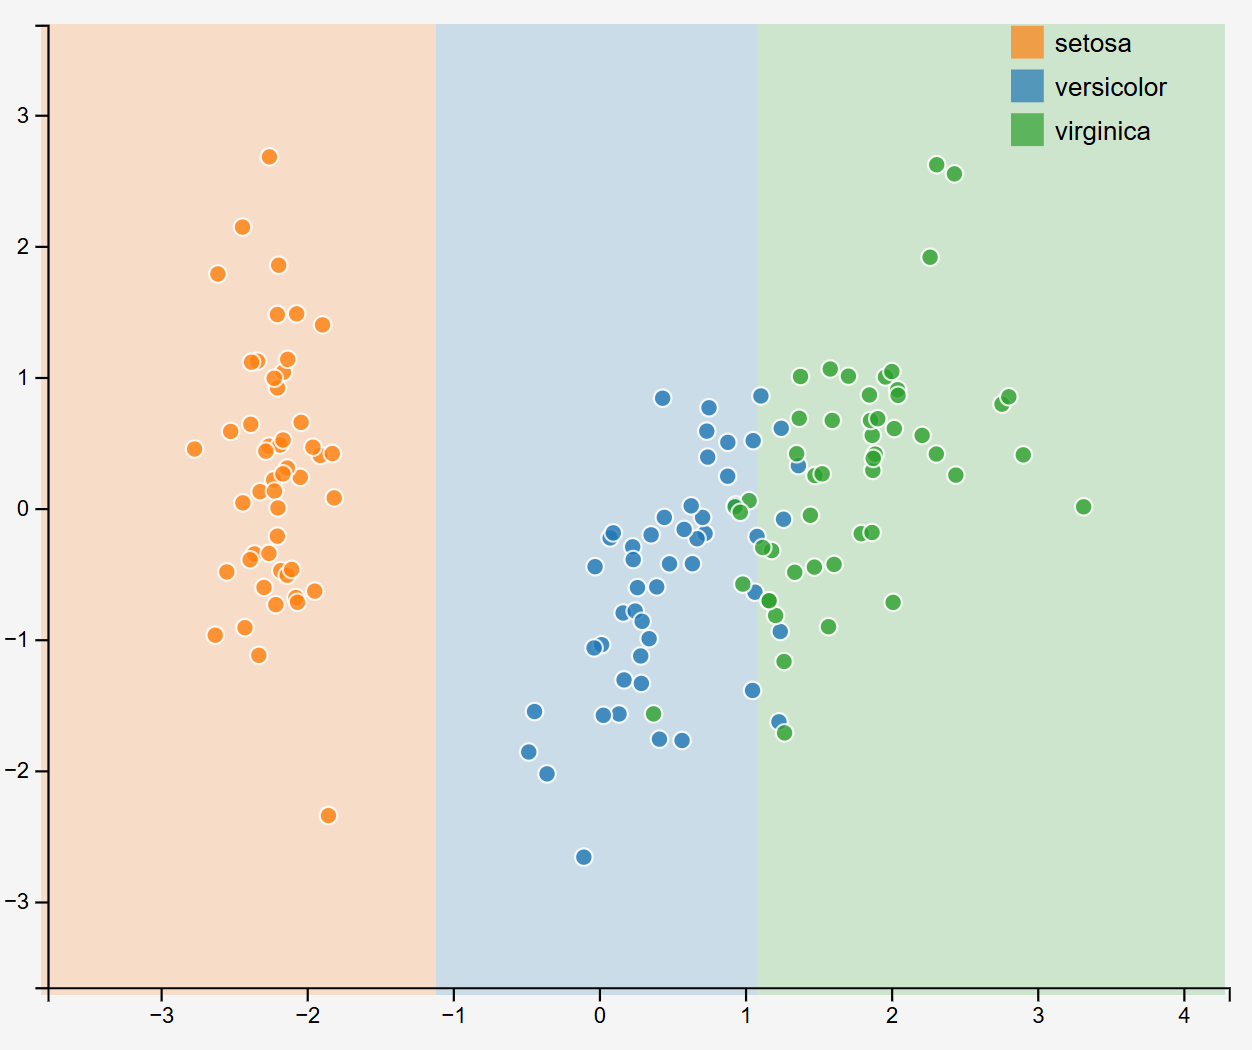
\includegraphics[width=0.7\linewidth]{images/first scatter plot.png}
    \caption{Initial spatial neighborhood analysis plot implementation using PCA projection with linear decision boundaries overlay for the iris dataset.}
    \label{fig:firstScatterPlot}
\end{figure}

We then developed a subsequent version of the spatial neighborhood analysis plot \cite{git4commit} that used a grid split for representing decision boundaries. As observed in Figure \ref{fig:secondScatterPlot}, this approach reveals subareas of the projected space that were not previously displayed. Additionally, we implemented hover interaction on spatial neighborhood analysis plot points, showing the point's class and additional information.

\begin{figure}
    \centering
    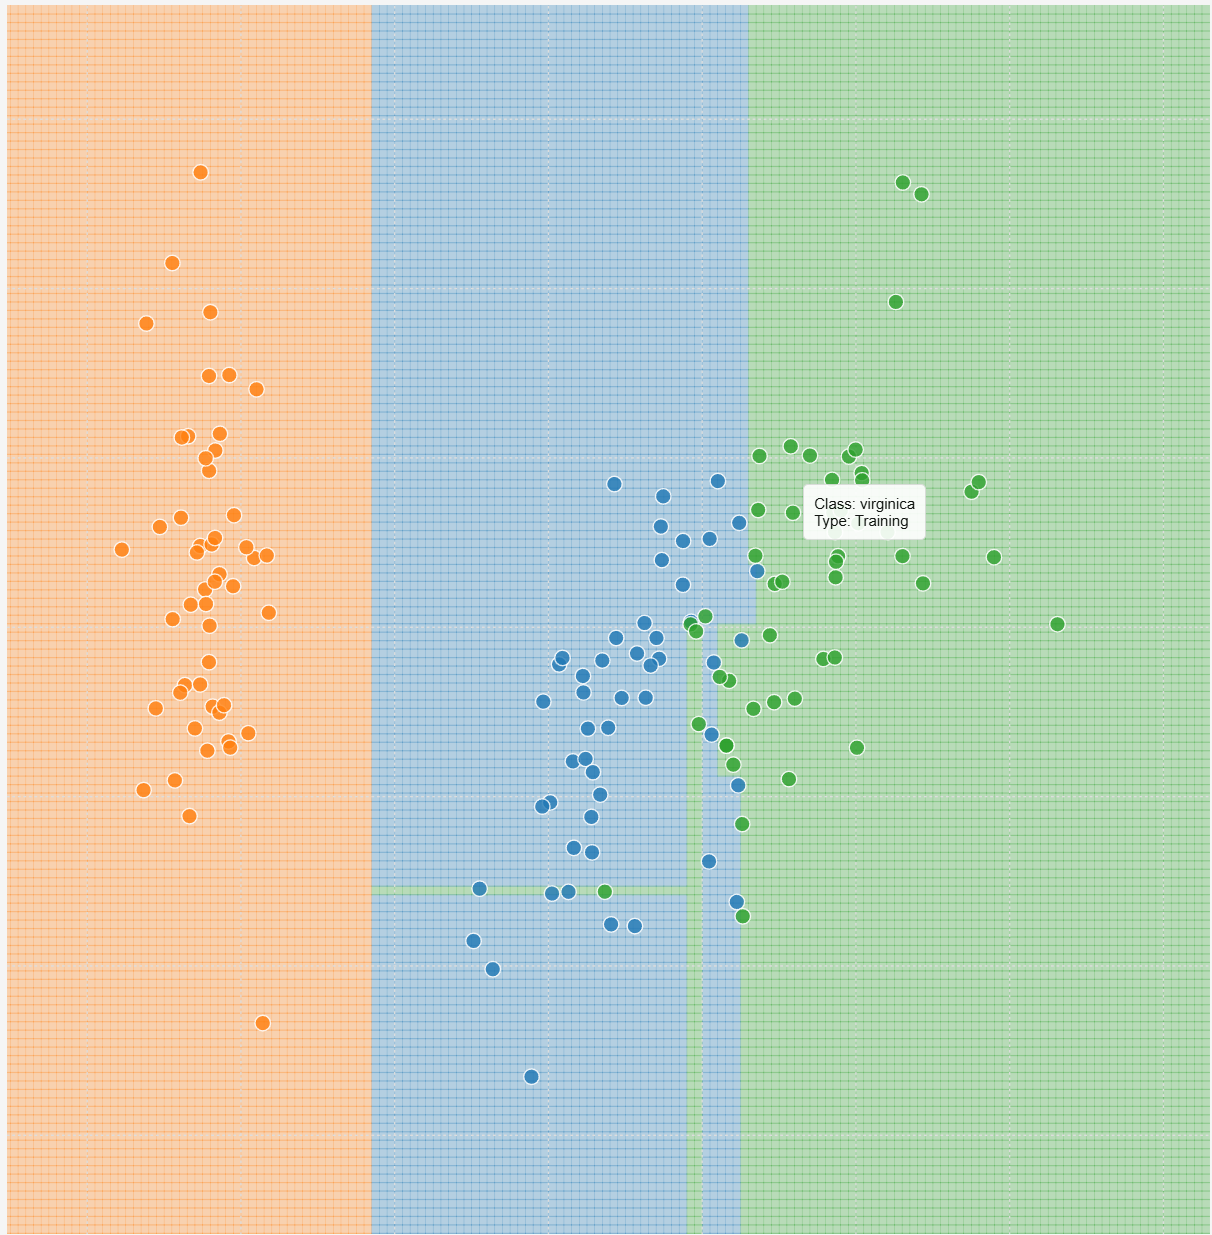
\includegraphics[width=0.6\linewidth]{images/second scatter plot.png}
    \caption{Enhanced spatial neighborhood analysis plot with grid-based decision boundary representation and interactive point tooltips.}
    \label{fig:secondScatterPlot}
\end{figure}

Regarding the decision boundaries representation implementation, we tested various approaches. The aforementioned grid was our first attempt, followed by an implementation \cite{git5commit} that used Ramer Douglas Peucker path approximation \cite{RAMER1972244, doi:10.3138/FM57-6770-U75U-7727} for simplifying decision paths in the projected space. Our final implementation \cite{git6commit} employs Voronoi tessellation \cite{Pokojski2018141150} with user settable granularity for space division.

This approach naturally accommodates the irregular decision boundaries produced by decision trees, unlike grid-based heatmaps that may introduce artificial discretization artifacts.

The algorithm begins by constructing a regular mesh grid that densely samples the 2D visualization space. The grid extends slightly beyond the actual data distribution, with boundaries defined as shown in Equation \ref{eq:PCABoundaries}.

\begin{equation}
\begin{aligned}
x_{\text{min}} &= \min(\mathbf{X}_{\text{2D}}[:, 0]) - 1, \quad x_{\text{max}} = \max(\mathbf{X}_{\text{2D}}[:, 0]) + 1 \\
y_{\text{min}} &= \min(\mathbf{X}_{\text{2D}}[:, 1]) - 1, \quad y_{\text{max}} = \max(\mathbf{X}_{\text{2D}}[:, 1]) + 1
\end{aligned}
\label{eq:PCABoundaries}
\end{equation}

where $\mathbf{X}_{\text{2D}}$ represents the PCA-transformed coordinates of all points in the synthetic neighborhood. This margin ensures that decision boundaries extending to the visualization edges are properly captured.

The mesh resolution is controlled by the \texttt{step} parameter, which defaults to 0.1 units. This creates a dense sampling with thousands of grid points as illustrated in Equation \ref{eq:PCAmeshResolution}.

\begin{equation}
\mathbf{G} = \{(x_i, y_j) \mid x_i \in [x_{\text{min}}, x_{\text{max}}], \, y_j \in [y_{\text{min}}, y_{\text{max}}], \, \text{step} = 0.1\}
\label{eq:PCAmeshResolution}
\end{equation}

The choice of step size represents a trade-off between boundary smoothness and computational efficiency. Smaller values produce smoother, more detailed boundaries but increase both computation time and the number of Voronoi cells requiring subsequent processing.

For each grid point $\mathbf{g} = (x, y)$ in the 2D visualization space, the surrogate model's prediction is determined. However, the decision tree operates in the original high-dimensional feature space, not in the reduced 2D space. This necessitates an inverse transformation shown in Equation \ref{eq:PCAinverseTransform}.

\begin{equation}
\mathbf{g}_{\text{original}} = S^{-1}(P^{-1}(\mathbf{g}))
\label{eq:PCAinverseTransform}
\end{equation}

where $P^{-1}$ represents the PCA inverse transformation and $S^{-1}$ represents the inverse standardization. PCA's linear nature makes this inverse transformation mathematically well-defined. The inverse PCA transformation reconstructs the original feature representation by multiplying the 2D coordinates by the transpose of the component matrix as illustrated in Equation \ref{eq:PCAReconstruction}.

\begin{equation}
\mathbf{x}_{\text{reconstructed}} = \mathbf{g} \cdot \mathbf{W}^T + \boldsymbol{\mu}
\label{eq:PCAReconstruction}
\end{equation}

where $\mathbf{W}$ contains the principal component vectors (eigenvectors of the covariance matrix) and $\boldsymbol{\mu}$ is the mean vector of the original data. The standardization is then inverted by rescaling using the stored standard deviations.

It is important to note that when PCA reduces dimensionality from $d$ dimensions to 2 dimensions, information in the $(d-2)$ discarded components is lost. The inverse transformation therefore reconstructs an approximation of the original point, with the reconstruction lying in the 2-dimensional subspace spanned by the first two principal components. 

Once grid points are transformed back to the original feature space, the surrogate model is used to generate the predictions.

This produces a class label for each grid point, effectively creating a discrete classification of the entire 2D visualization space according to how the decision tree would classify points in those regions. The resulting prediction array $\mathbf{Z}$ has the same shape as the original mesh grid, with each element containing the predicted class label for the corresponding spatial location.

The \texttt{scipy.spatial.Voronoi} class constructs the initial tessellation by computing the Voronoi diagram for all grid points. Each grid point becomes a Voronoi site, and the diagram partitions the plane into cells such that every location within a cell is closer to that cell's site than to any other site. The Voronoi construction returns:

\begin{itemize}
    \item \textbf{Vertices}: The corner points where Voronoi cell boundaries meet
    \item \textbf{Regions}: Lists of vertex indices defining each Voronoi cell polygon
    \item \textbf{Ridge points}: Pairs of sites that share a boundary
\end{itemize}

Each Voronoi region is converted to a Shapely Polygon object for geometric manipulation. 
Infinite regions (those extending to infinity, indicated by vertex index $-1$) are filtered out since these lie outside the bounded visualization area and cannot be meaningfully rendered.

The raw Voronoi tessellation produces one cell per grid point, resulting in thousands of tiny polygons. Since adjacent grid points often receive the same class prediction from the decision tree, these cells are merged into larger, unified regions using graph-based connectivity analysis.

The undirected graph $G = (V, E)$ is constructed, where: \textbf{Vertices} $V$ represent Voronoi regions and \textbf{Edges} $E$ connect adjacent regions that share the same predicted class.

Two regions are connected if they share a ridge (common boundary) in the Voronoi diagram and their corresponding grid points received identical class predictions from the decision tree.
Using NetworkX, all connected components in this graph are identified. Each connected component represents a maximal set of Voronoi cells that are both spatially adjacent and classified identically. For each component, all constituent polygons are merged into a single unified region using Shapely's \texttt{unary\_union} operation.

The backend transmits the merged polygon boundaries as arrays of vertex coordinates to the frontend. These polygons are then rendered on the webpage.
Each polygon is filled with a color corresponding to its predicted class, maintaining visual consistency with the color encoding used for scatter plot points. 

The Voronoi approach provides several advantages for our visualization requirements. It naturally handles irregular decision boundaries without imposing artificial geometric constraints, unlike approaches that force rectangular partitions. The graph-based merging also produces clean, consolidated regions that match the decision tree's actual partitioning structure, avoiding visual clutter from excessive fragmentation. On top of that the method scales efficiently: while grid generation is $O(n^2)$ in the number of grid cells, the Voronoi construction and merging operations remain computationally tractable for interactive use. One can observe an example of the final result in Figure \ref{fig:scatterplotvoronoi}

\begin{figure}
    \centering
    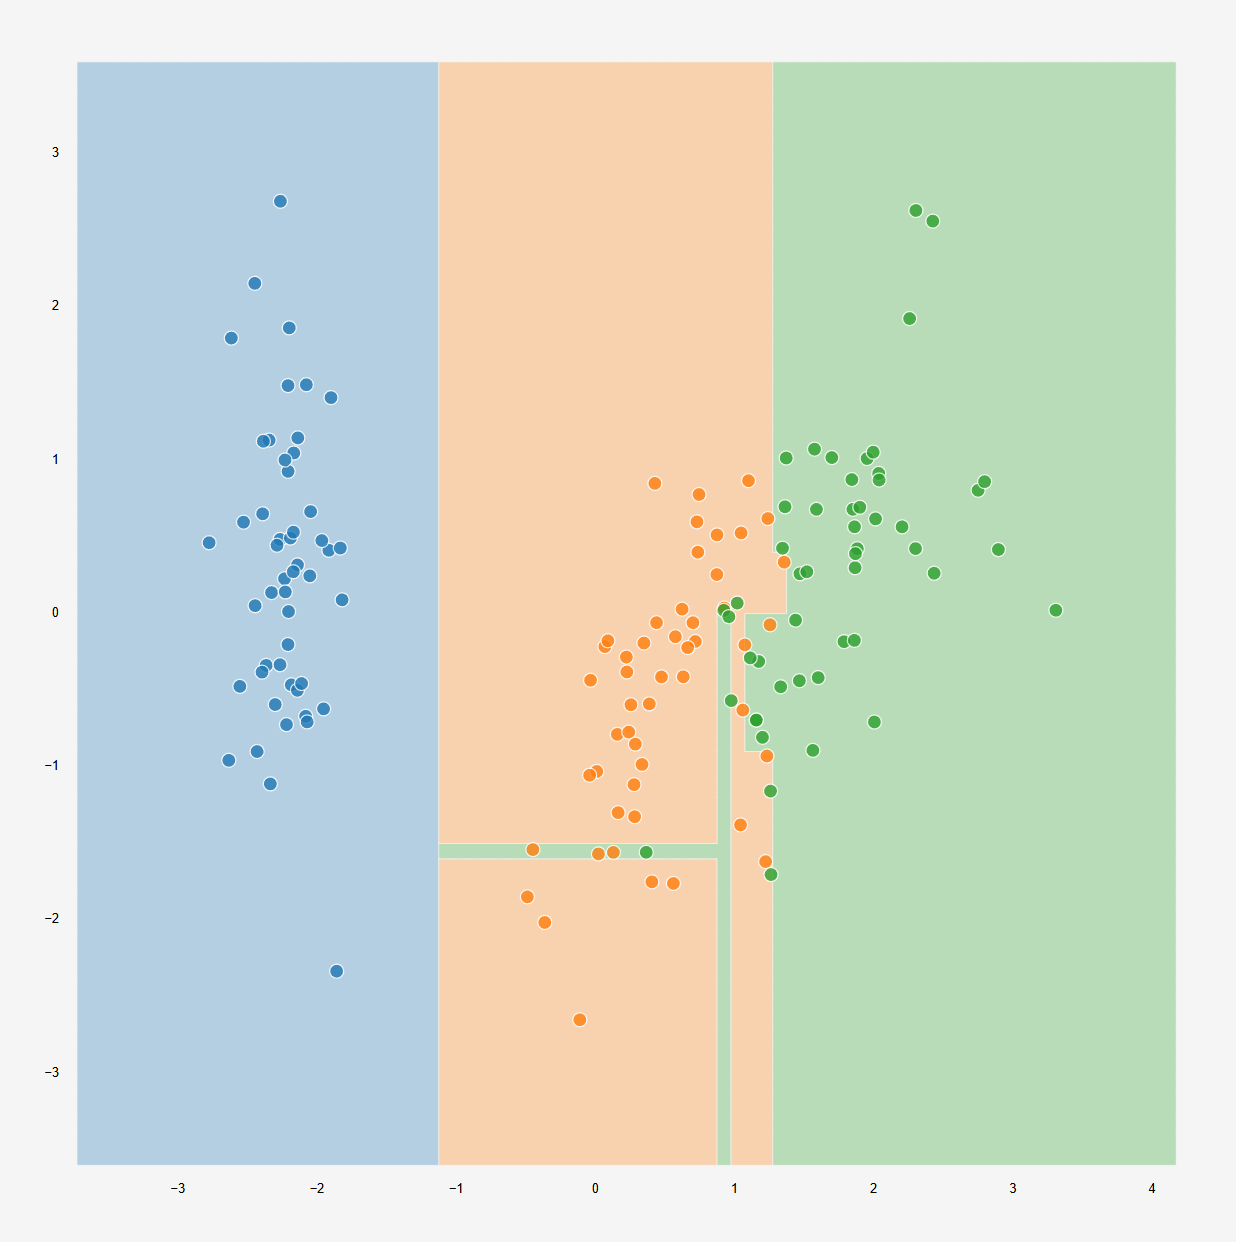
\includegraphics[width=0.6\linewidth]{images/third scatter plot voronoi.png}
    \caption{Final spatial neighborhood analysis plot implementation featuring Voronoi tessellation-based decision boundaries with user-configurable granularity.}
    \label{fig:scatterplotvoronoi}
\end{figure}

Later in the project development, we added the option to switch between the initially default PCA and t-SNE \cite{git18commit}, along with UMAP and MDS \cite{git19commit}. To enable users to switch between the four dimensionality reduction techniques, we implemented buttons with related names \cite{git20commit} and added highlighting of split node descendants \cite{git21commit}. 

Considering the possibility of datasets with more than ten classes, we implemented RGB space projection for color classes \cite{git24commit}. We later replaced this with a projection in the CIELAB a*-b* (L*=70) color space \cite{git29commit}. The issue with RGB space is that it is three-dimensional, while dimensionality reduction projections are two-dimensional. The relevant implementation does not differ significantly. Additionally, we added the option for showing the original dataset in the projected space. Points from the original dataset are represented with lower opacity to distinguish them from the generated neighborhood ones \cite{git25commit}.

All the features just discussed are shown in Figure \ref{fig:webappswitchdimensionalityandSplitNodeHighANdVarious}. As observed, decision boundaries are not present in the UMAP projection since UMAP, t-SNE, and the used MDS are non-linear projections, and the same results as for PCA cannot be directly achieved. The colors are also the RGB-projected ones, even though the dataset used for showcasing functionality (iris) contains only three classes.

\begin{figure}[h]
    \centering
    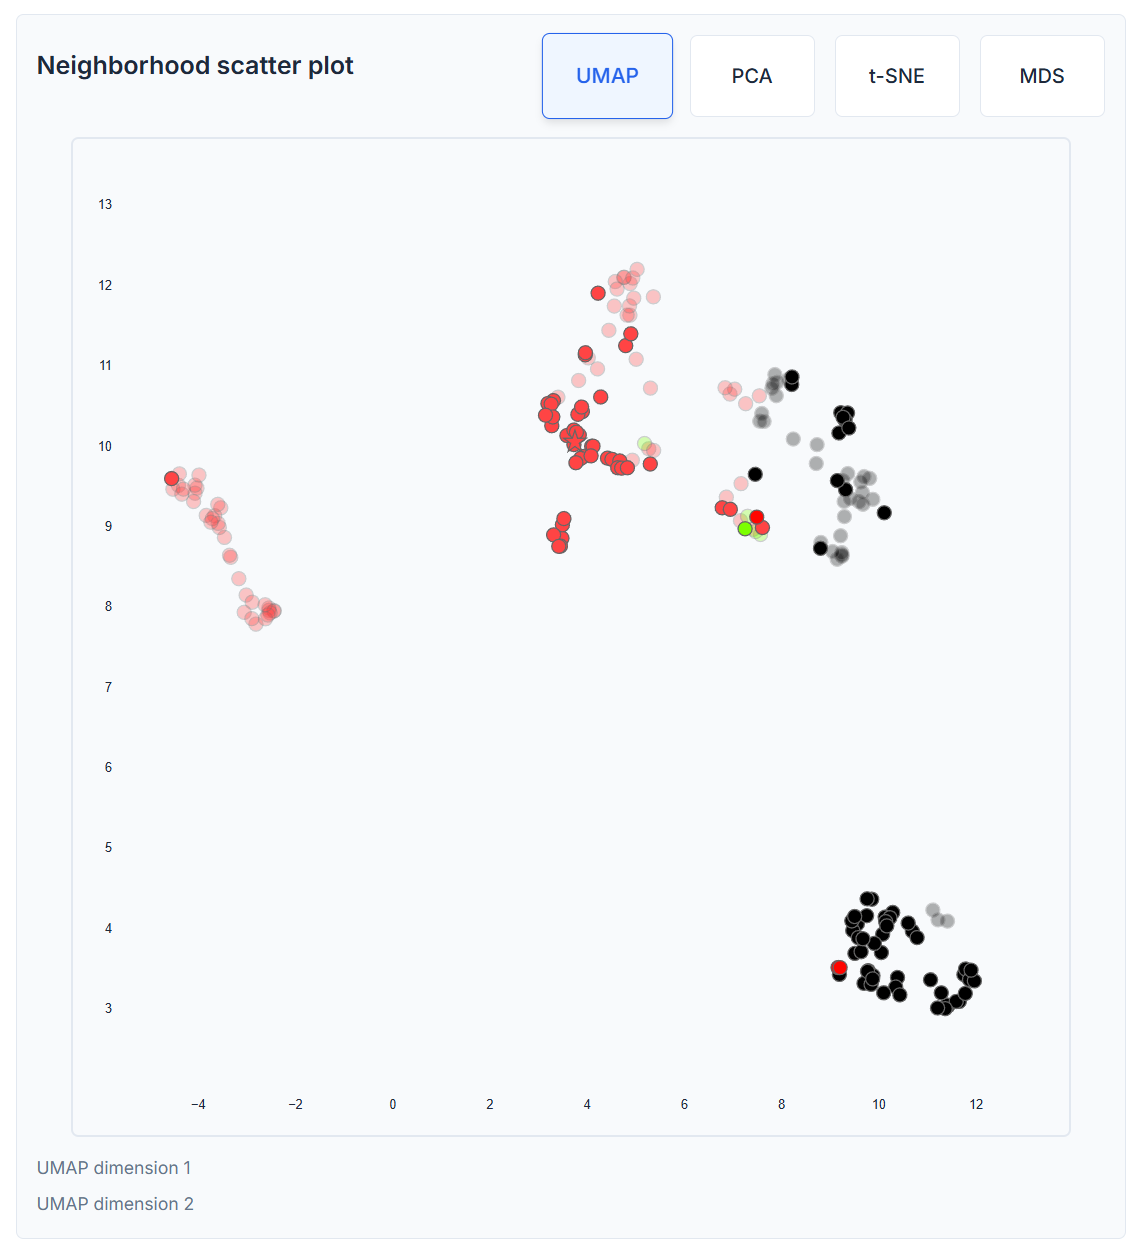
\includegraphics[width=0.6\linewidth]{images/DR switch and descendant highlight and various webapp.png}
    \caption{Advanced webapp features including dimensionality reduction technique selection (UMAP shown), RGB color space projections and original dataset overlay with opacity differentiation.}
    \label{fig:webappswitchdimensionalityandSplitNodeHighANdVarious}
\end{figure}

Regarding the projection in the CIELAB space, this approach addresses the challenge of generating distinct colors for datasets with numerous classes (more than ten). Unlike predefined color palettes that become inadequate for high-cardinality classification problems, this method dynamically generates colors based on the data distribution.

The algorithm operates on class centroids in the original feature space. For each class $c$, the centroid $\boldsymbol{\mu}_c$ is computed as the mean of all samples belonging to that class:

\begin{equation}
\boldsymbol{\mu}_c = \frac{1}{|\mathcal{X}_c|} \sum_{\mathbf{x}_i \in \mathcal{X}_c} \mathbf{x}_i
\end{equation}

where $\mathcal{X}_c$ denotes the set of all samples with class label $c$.

These high-dimensional centroids are then projected into two-dimensional space using the same dimensionality reduction method and parameters employed for the scatter plot visualization (PCA, t-SNE, UMAP, or MDS). This ensures consistency between the spatial layout of the scatter plot and the color assignments. The projected coordinates are normalized to the $[0, 1]$ range using min-max scaling.

The normalized 2D coordinates $(x, y) \in [0, 1]^2$ are mapped to the chromatic dimensions of the CIELAB color space. CIELAB is a perceptually uniform color space designed to approximate human vision, where the $L^*$ dimension represents lightness, and the $a^*$ and $b^*$ dimensions represent the green-red and blue-yellow color opponents, respectively. The mapping is defined as:

\begin{equation}
\begin{aligned}
L^* &= 70 \\
a^* &= ((x - 0.5) \times 2) \times 128 \\
b^* &= ((y - 0.5) \times 2) \times 128
\end{aligned}
\end{equation}

The lightness value is fixed at $L^* = 70$ to ensure consistent brightness across all generated colors, avoiding very dark or very light hues. The $(x, y)$ coordinates are centered at $(0.5, 0.5)$, scaled to $[-1, 1]$, and then multiplied by 128 to span the typical range of CIELAB's chromatic dimensions.
The CIELAB coordinates are subsequently converted to hexadecimal color strings for web rendering.

The key advantage of CIELAB over direct RGB projection lies in its perceptual uniformity: equal distances in CIELAB space correspond to approximately equal perceived color differences. This property ensures that classes with similar feature distributions receive visually similar colors, while dissimilar classes are assigned perceptually distinct colors. Additionally, CIELAB's chromatic plane $(a^*, b^*)$ is naturally two-dimensional, making it ideally suited for mapping 2D projections without the dimensional mismatch that occurs with three-dimensional RGB space.

In figure \ref{fig:colorsProjection}, one can observe both the CIELAB a*-b* (L*=70) and RGB color spaces, and, for each, an the example projection of the mean instances of each class present in the iris dataset.

\begin{figure}
    \centering
    % Row 1
    \begin{subfigure}[c]{0.45\textwidth}
        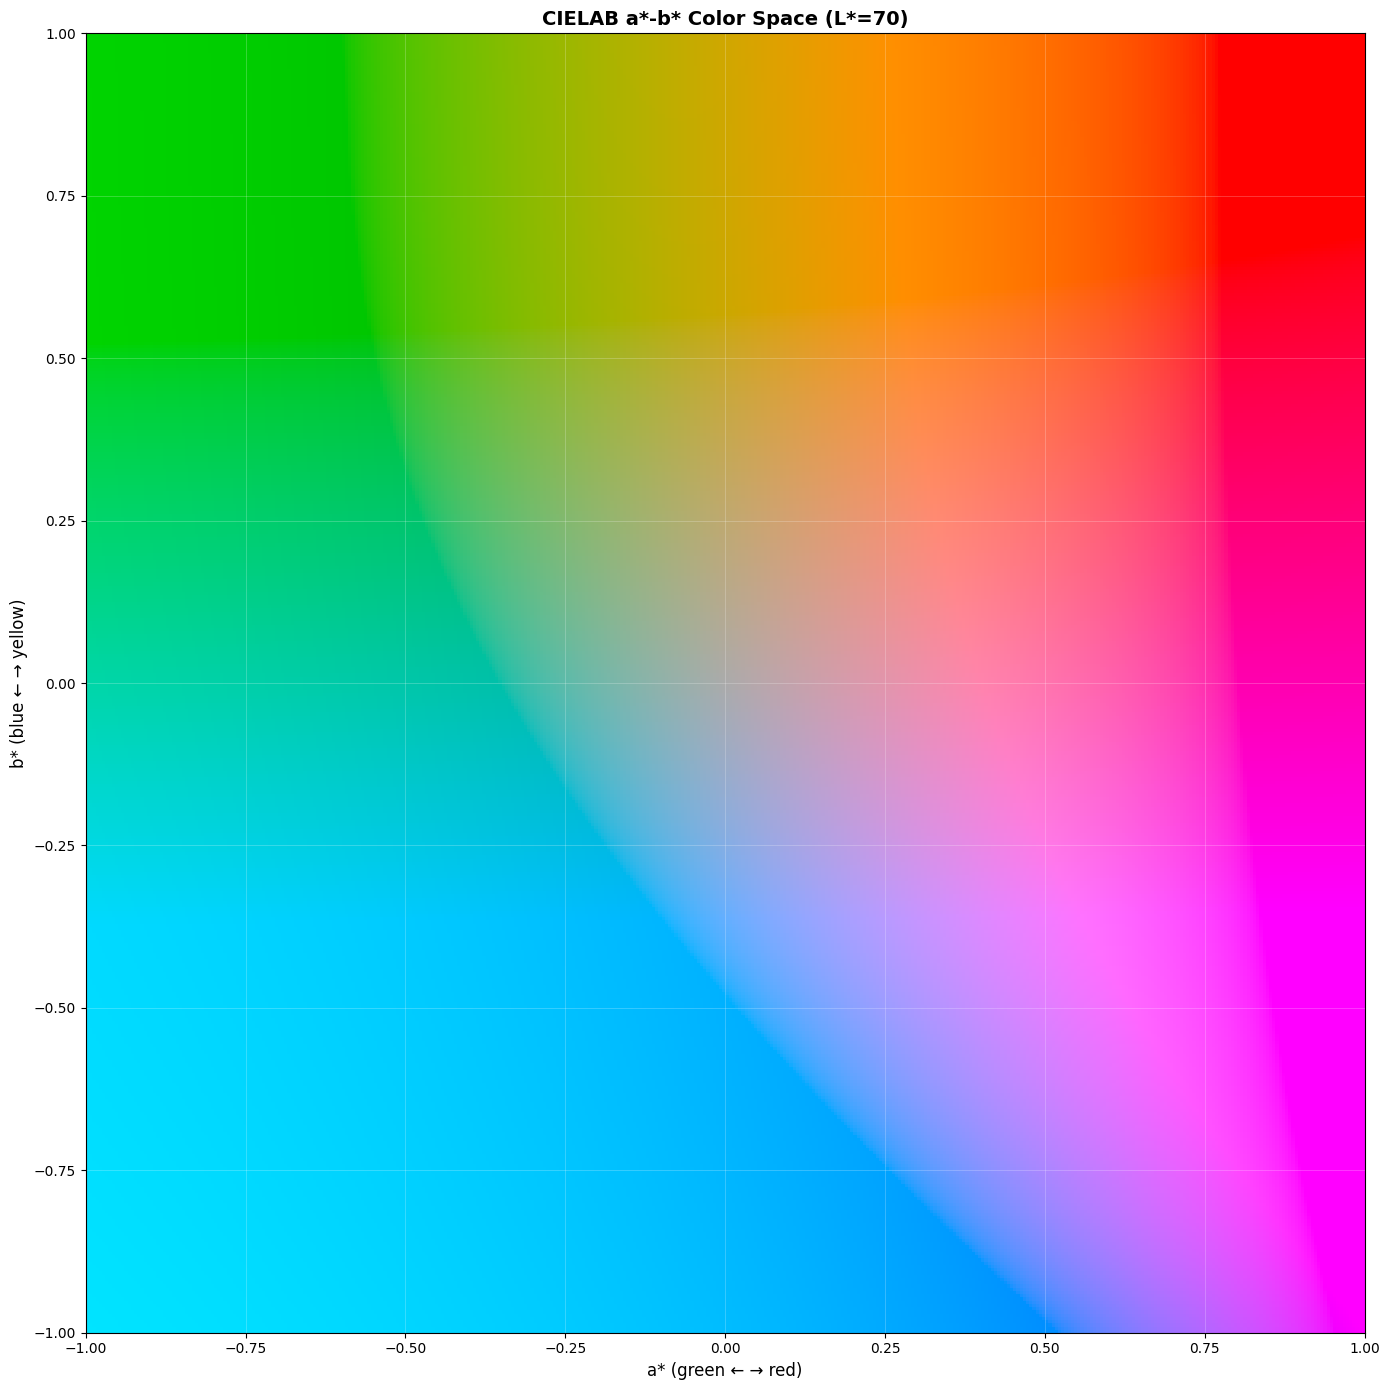
\includegraphics[width=\textwidth]{images/CIELAB a-b Color Space (L=70).png}
        \caption{CIELAB a-b Color Space with Luminosity fixed at 70}
    \end{subfigure}
    \hfill
    \begin{subfigure}[c]{0.45\textwidth}
        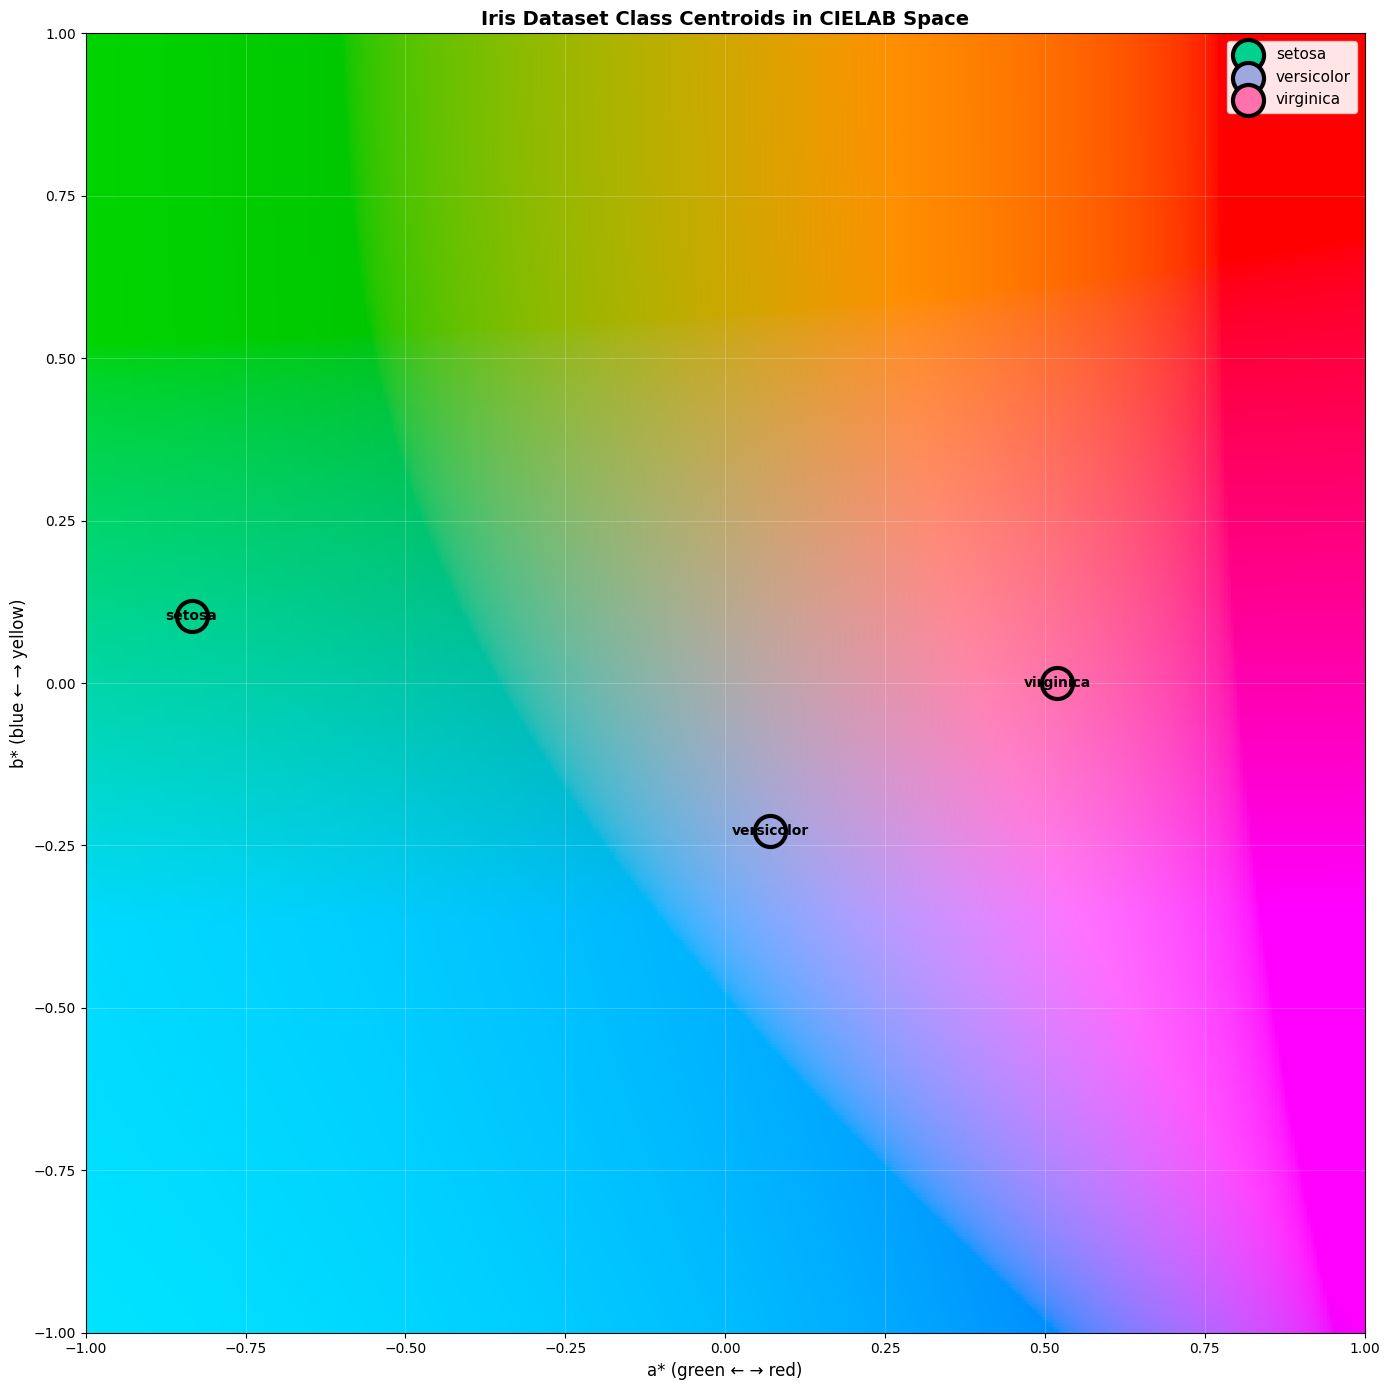
\includegraphics[width=\textwidth]{images/Iris Dataset Class Centroids in CIELAB Space.png}
        \caption{Iris Dataset Class Centroids projected in the CIELAB a*-b* L=70 Color Space.}
    \end{subfigure}

    \vspace{0.5cm} % space between rows

    % Row 2
    \begin{subfigure}[c]{0.45\textwidth}
        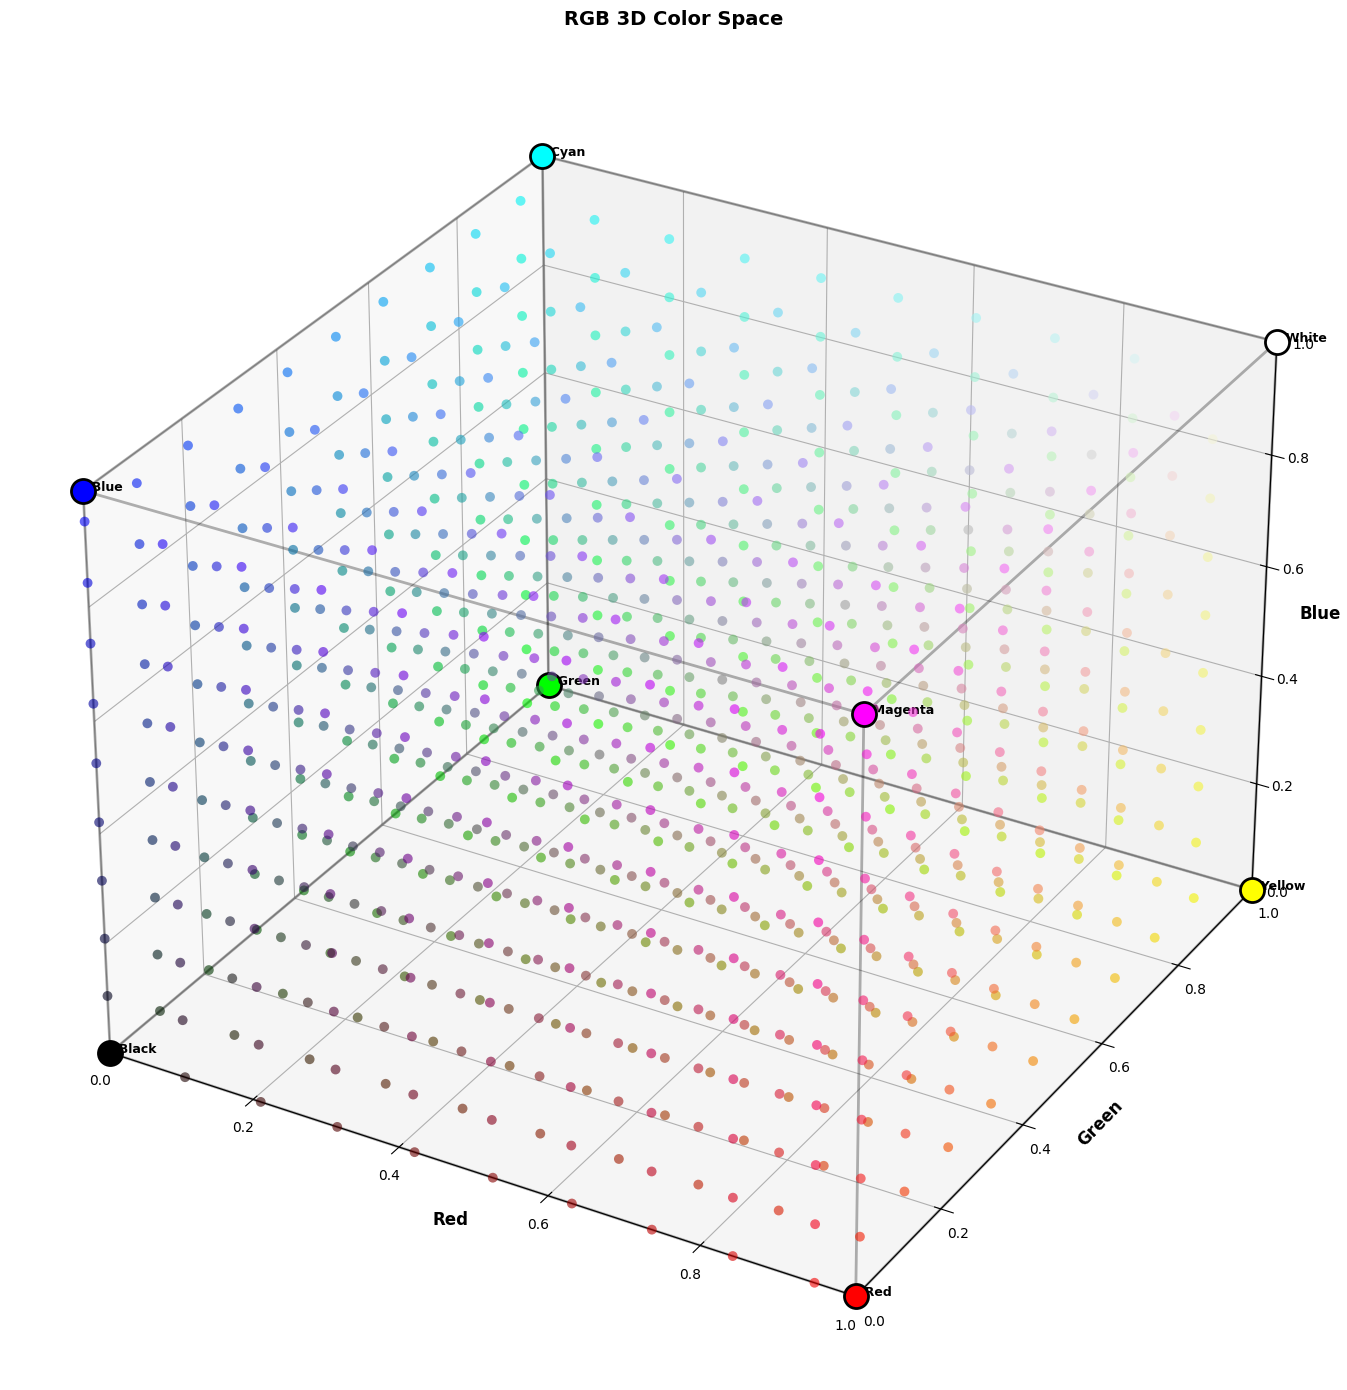
\includegraphics[width=\textwidth]{images/RGB 3D Color Space.png}
        \caption{RGB 3D Color Space.}
    \end{subfigure}
    \hfill
    \begin{subfigure}[c]{0.45\textwidth}
        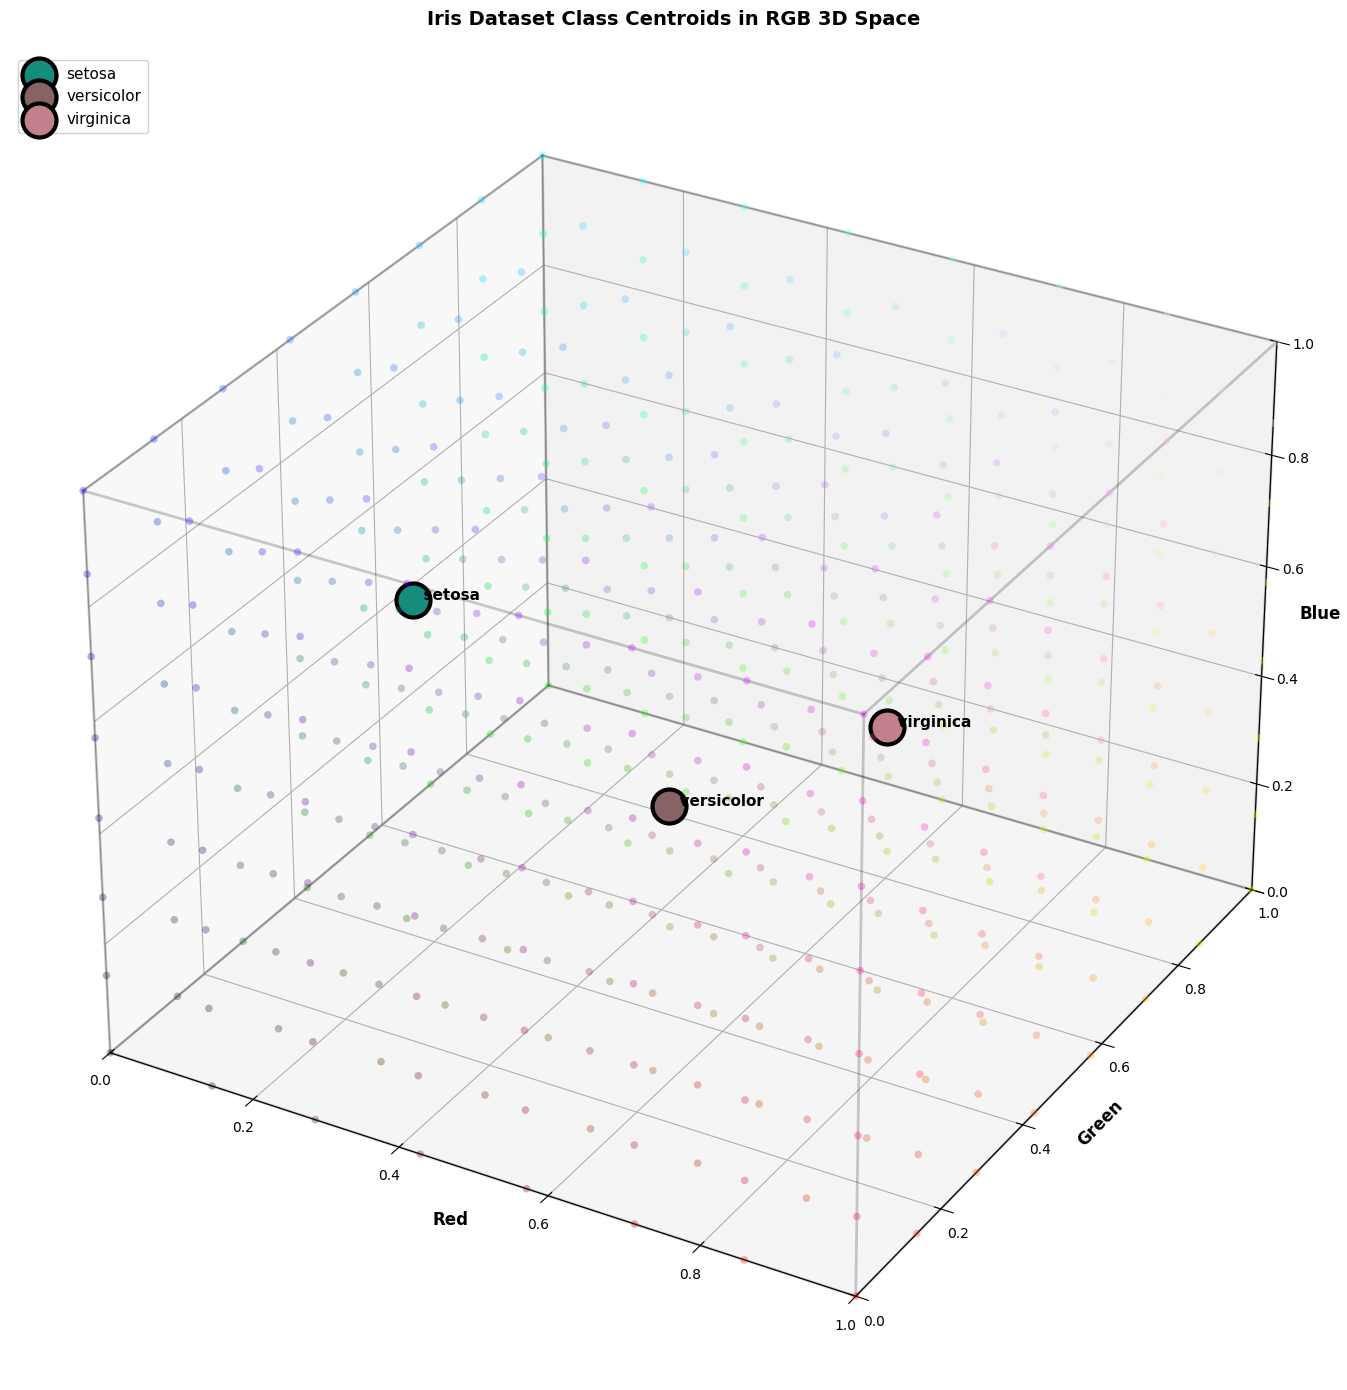
\includegraphics[width=\textwidth]{images/Iris Dataset Class Centroids in RGB 3D Space.png}
        \caption{Iris Dataset Class Centroids projected in the RGB 3D Color Space}
    \end{subfigure}

    \caption{Colors projection that were considered during development.}
    \label{fig:colorsProjection}
\end{figure}

\subsection{Tree layout}

We began the project development with the first implementation of the surrogate model plot \cite{git1commit}. Initially, our main focus centered on creating a visualization that could represent all possible trees in a polished manner.

The primary challenge involved node positioning; using a fixed angle for all splits at different tree heights and with varying numbers of subtrees would have resulted in overlapping nodes.

As observed in Figure \ref{fig:earlyProtoypeDecisionTreeVisualization}, which represents a section of the complex tree structure used for testing at this development stage, we successfully tested and accomplished node positioning at both labyrinthine and elementary levels of tree complexity.

\begin{figure}
    \centering
    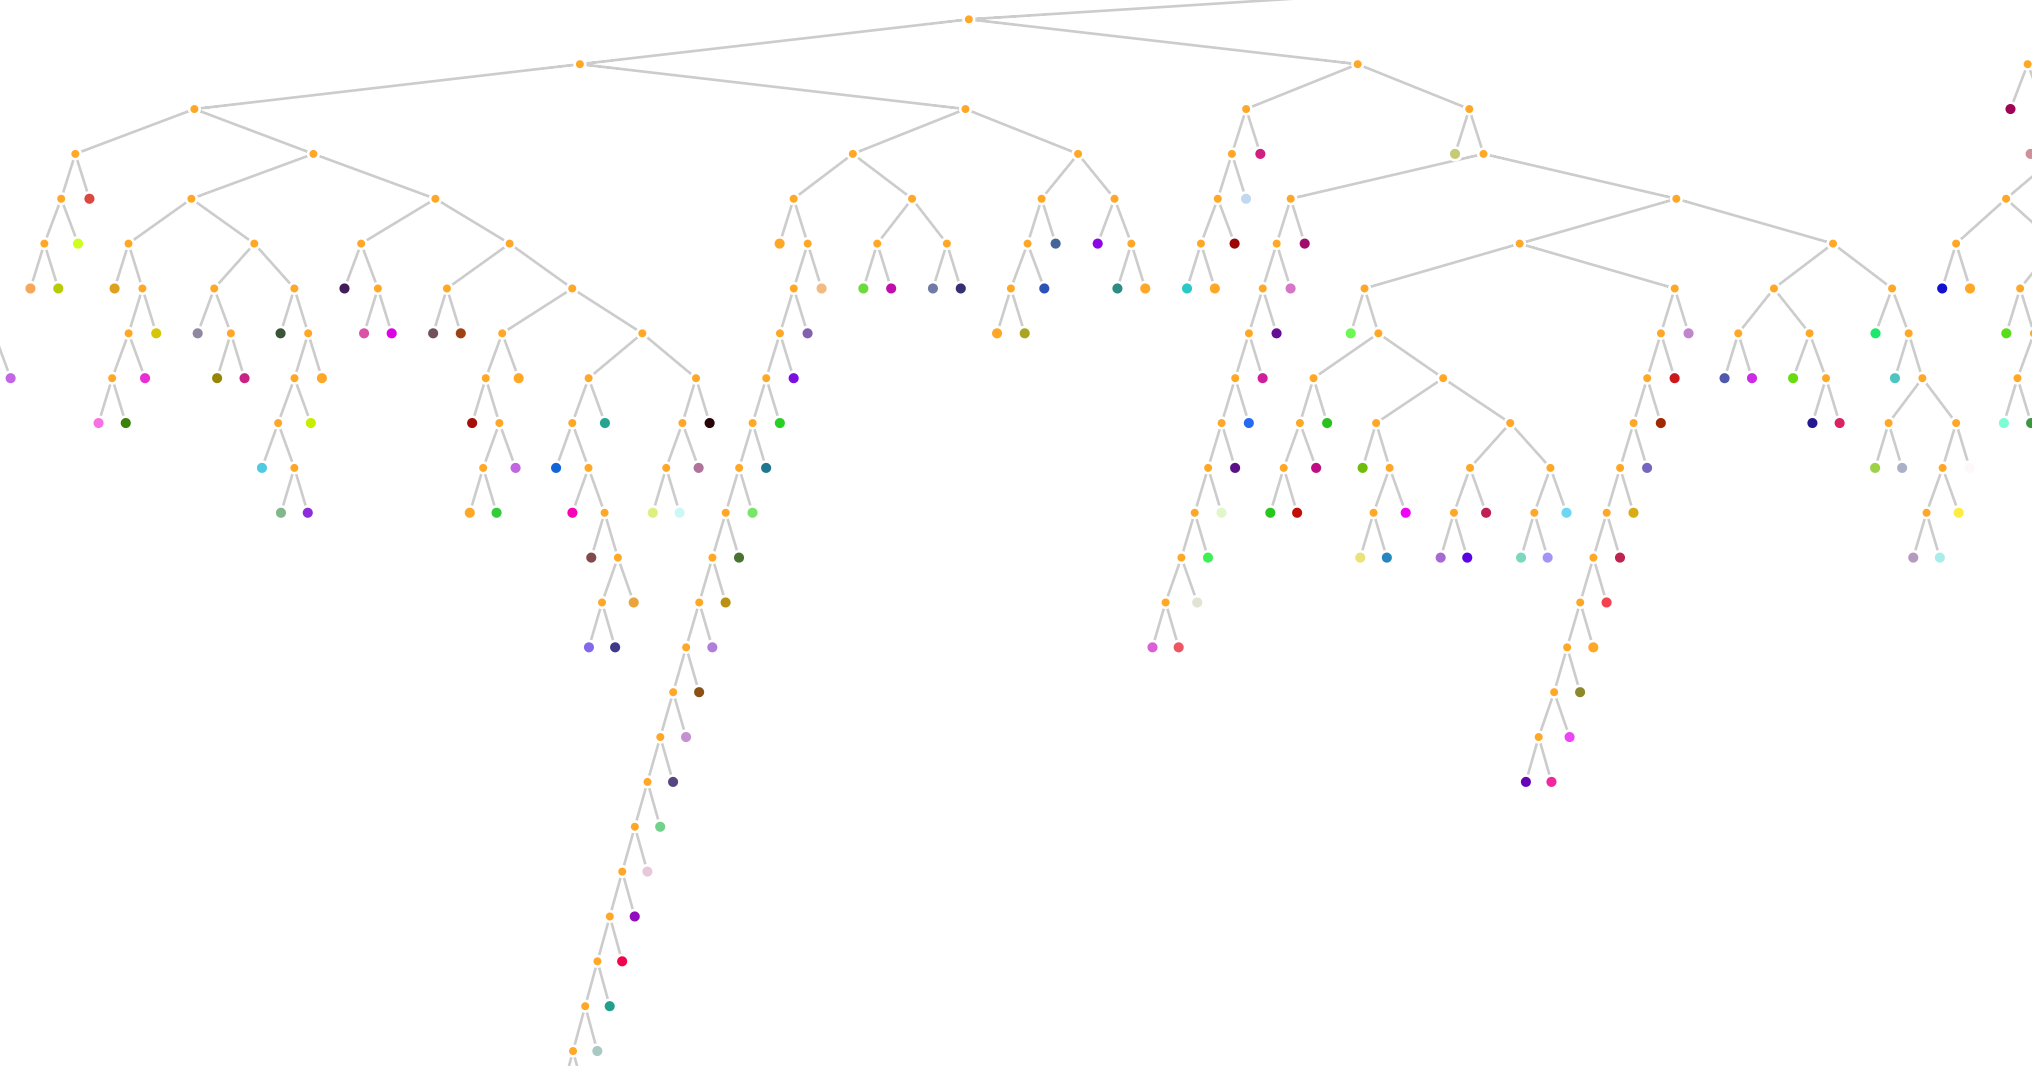
\includegraphics[width=\linewidth]{images/early protoype of decision tree visualization.png}
    \caption{Initial surrogate model visualization prototype demonstrating node positioning algorithm for complex tree structures without overlap.}
    \label{fig:earlyProtoypeDecisionTreeVisualization}
\end{figure}

The node positioning algorithm employs D3's hierarchical tree layout, which implements the Reingold-Tilford algorithm \cite{1702828} for creating tidy tree drawings. This algorithm ensures optimal node placement without overlaps through three key mechanisms.

The layout dynamically scales the available space based on tree complexity. Both horizontal and vertical dimensions are calculated proportionally to the total number of nodes: $horizontalSpacing = n_{nodes} \times minSplitWidth$ and $verticalSpacing = n_{nodes} \times minSplitHeight$, where $minSplitWidth = 30$ pixels and $minSplitHeight = 25$ pixels. 

This adaptive scaling ensures that larger trees receive proportionally more space, preventing visual congestion.
On top of that a separation function enforces consistent inter-node spacing throughout the tree structure. Set to $2 \times minSplitWidth = 60$ pixels, this separation value creates uniform gaps between adjacent nodes at the same depth level, maintaining visual clarity regardless of the local branching structure.

The layout coordinates also undergo an initial transform calculation that fits the entire tree within the viewport bounds while preserving aspect ratio. This transform computes optimal scale factors for both dimensions and applies appropriate translations to center the tree, enabling users to immediately view the complete structure. The system then applies zoom and pan capabilities, allowing detailed exploration of specific regions while maintaining the overall spatial relationships established by the Reingold-Tilford algorithm.

The next implementation step \cite{git2commit} involved implementing click-on-leaf-node interaction for path tracing from the root node to the clicked leaf, as demonstrated in Figure \ref{fig:Root-to-leaf}. Additionally, we built hover interactions for split and leaf nodes to display either the leaf node class or the split condition based on the node type being hovered, as shown in Figures \ref{fig:split-tooltip} and \ref{fig:leaf-tooltip}.

\begin{figure}[htbp]
    \centering
    \begin{subfigure}[c]{0.6\textwidth}
        \centering
        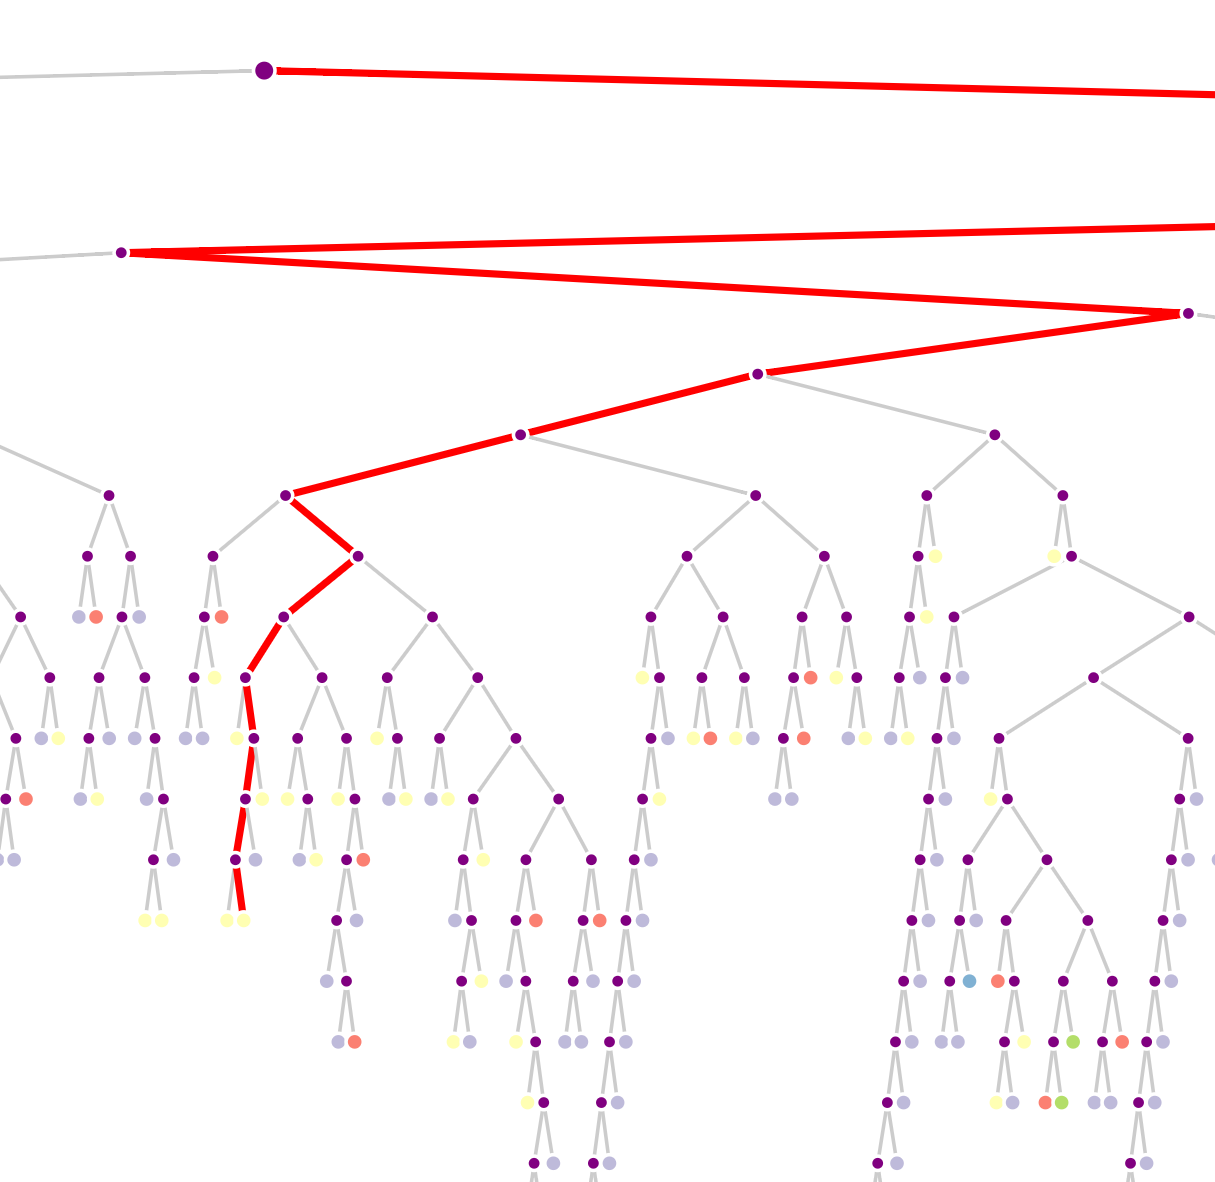
\includegraphics[height=\textwidth]{images/first highlight on click.png}
        \caption{Root to leaf node path tracing example.}
        \label{fig:Root-to-leaf}
    \end{subfigure}%
    \hspace{0.05\textwidth}%
    \begin{subfigure}[c]{0.3\textwidth}
        \centering
        \begin{subfigure}[c]{\textwidth}
            \centering
            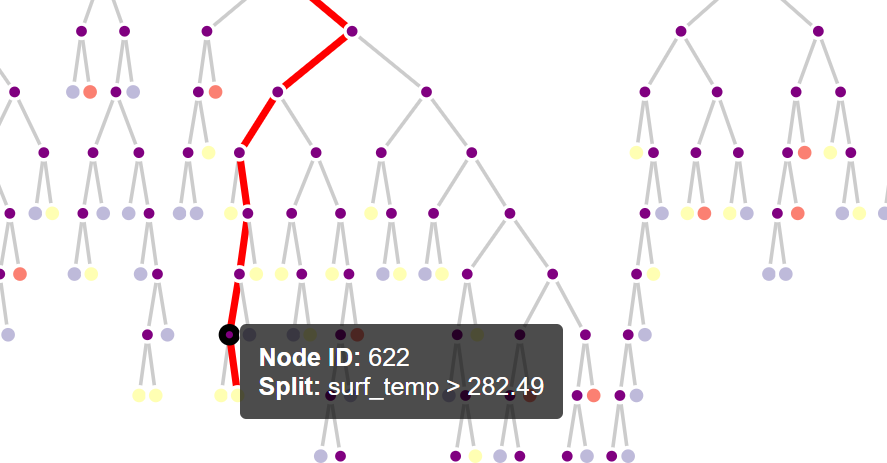
\includegraphics[width=\textwidth]{images/first tooltip split node.png}
            \caption{Tooltip on split node showing the split condition.}
            \label{fig:split-tooltip}
        \end{subfigure}
        
        \vspace{0.02\textheight}
        
        \begin{subfigure}[c]{\textwidth}
            \centering
            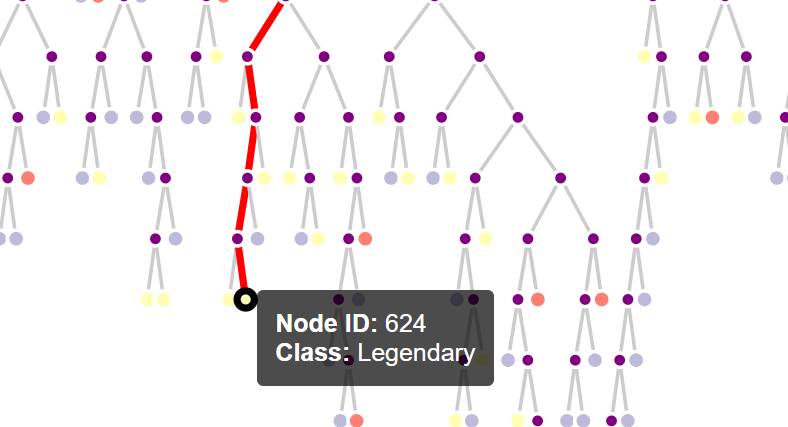
\includegraphics[width=\textwidth]{images/first tooltip node.png}
            \caption{Tooltip on leaf node showing its class.}
            \label{fig:leaf-tooltip}
        \end{subfigure}

    \end{subfigure}
    \caption{Enhanced surrogate model prototype with interactive features: path highlighting and contextual tooltips for different node types.}
\end{figure}

Subsequently, as shown in Figure \ref{fig:constantHighlightTree}, we added a first version of constant highlighting of the explained instance path in the surrogate model plot \cite{git22commit} and embedded sklearn information regarding split nodes \cite{git23commit} (namely: feature index, impurity, samples, and class distribution).

\begin{figure}
    \centering
    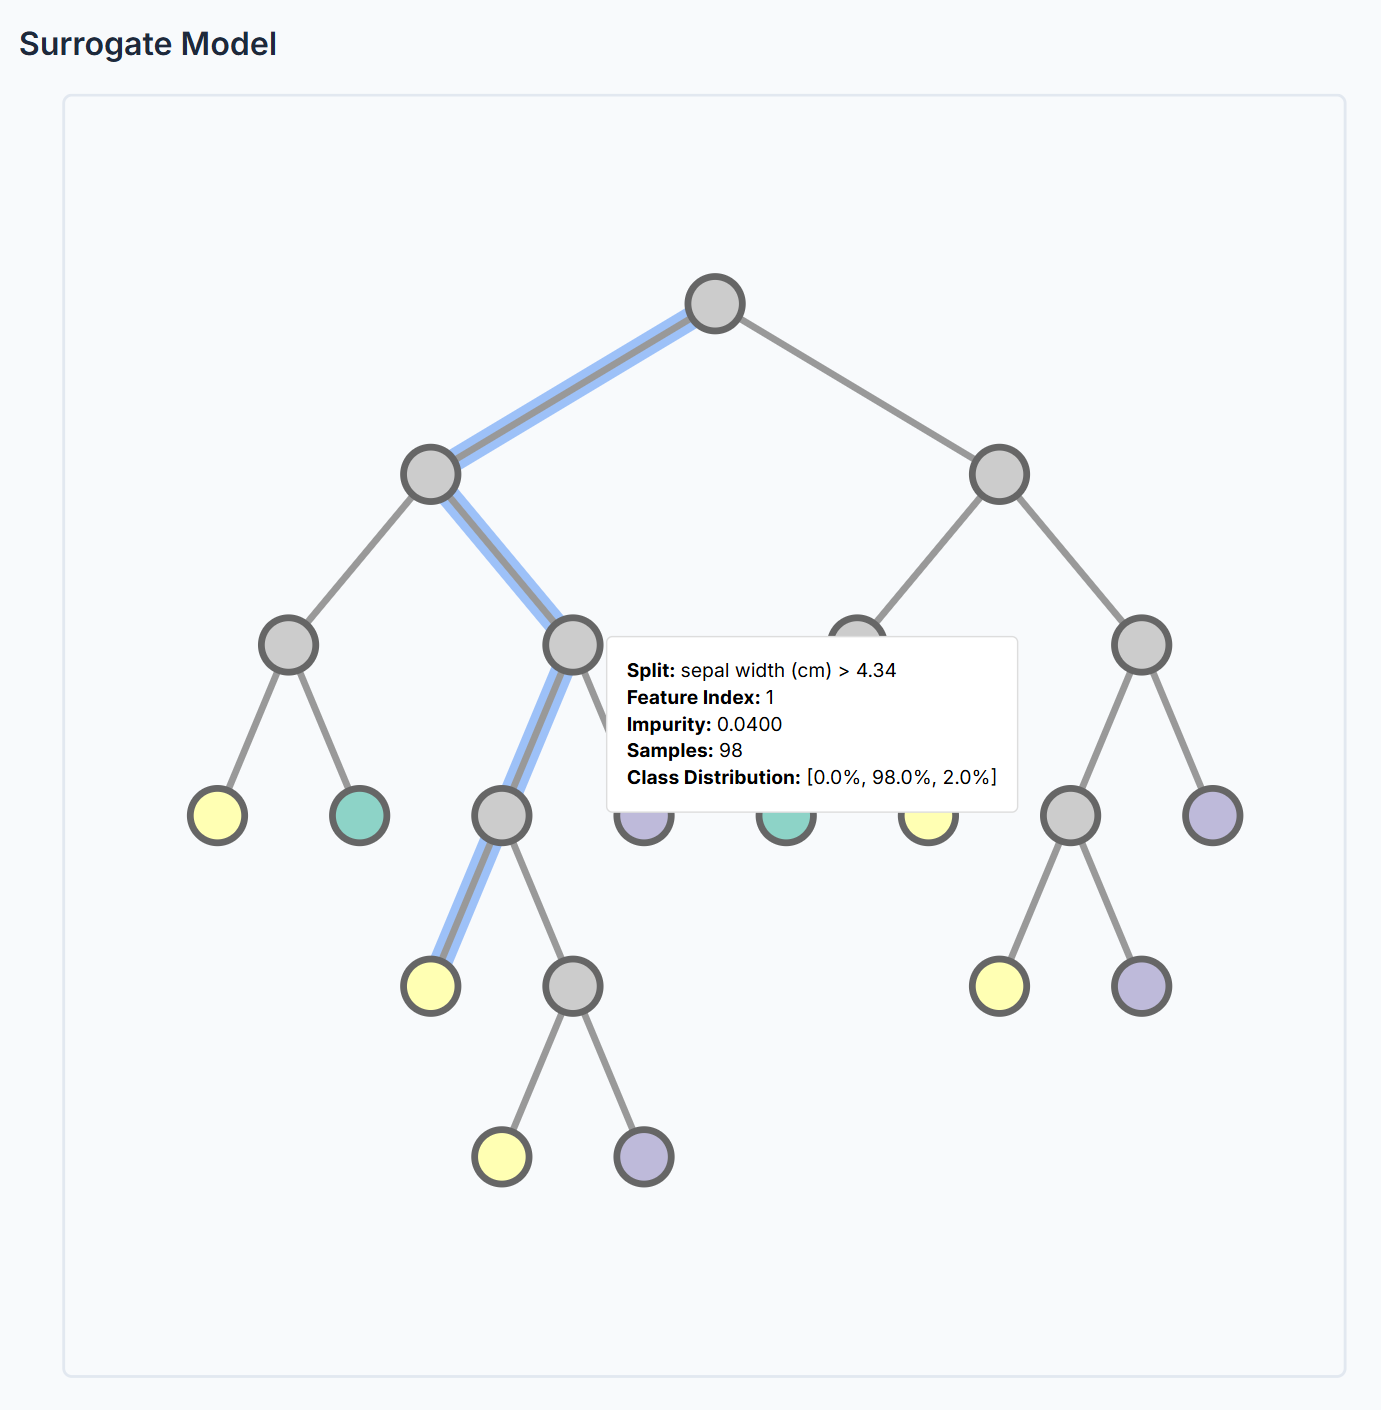
\includegraphics[width=0.5\linewidth]{images/Costant highlight and new tooltip tree basic.png}
    \caption{Constant highlighting of the explained instance path in the surrogate model and new tooltip}
    \label{fig:constantHighlightTree}
\end{figure}

\subsection{Rule centered approaches}

While the classical tree layout successfully visualizes the complete structure of the surrogate decision tree and provides interactive features for path exploration, we recognized that it presents inherent limitations for rule-focused analysis. Although users can trace decision paths by clicking on leaf nodes and examining individual split conditions through tooltips, the hierarchical layout, especially in complex surrogate models, requires significant cognitive effort to identify the generated rule and counterrules. 
The traditional top-down structure, while effective for understanding the overall tree topology and decision flow, necessitates visual scanning across multiple tree levels and mental aggregation of conditions along a path, a process that becomes increasingly challenging as tree depth and complexity grow.

Moreover, the classical layout allocates equal visual prominence to all branches of the decision tree, regardless of their relevance to the explained instance. This representation, while democratic, does not prioritize the specific rule that explains the instance of interest, nor does it facilitate direct comparison between factual rules and their counterfactual counterparts. 

In response to these limitations, we developed two complementary rule-centered visualizations, temporarily named \texttt{Tree Spawn} and \texttt{Blocks} layouts, and later renamed \texttt{Rules Centered} and \texttt{Rule Centered and Rule and Counterfactual Centered} respectively. These approaches maintain the interpretability benefits of tree-based hierarchical representations while reorganizing the visual presentation to prioritize rule comprehension, minimize cognitive load for path interpretation, and facilitate direct exploration of the relationships between factual explanations and counterfactual alternatives. The following subsub-sections
% \ref{subsubsec:tree spawn} and \ref{subsubsec:blocks} 
detail the design and briefly discuss the implementation of each approach.

\subsubsection{Rules Centered layout}
% \label{subsubsec:tree spawn}

% Later, our development moved toward implementing two new surrogate model visualizations, temporarily named "tree spawn" and "blocks". 
The first implementation of the Rules Centered layout \cite{git26commit} can be seen in Figure \ref{fig:Tree spawn first implementation}, where we represent the explained instance path as rectangles with tooltip information embedded within them instead of using circles, which are used for other branches of the surrogate model tree.

\begin{figure}[h]
    \centering
    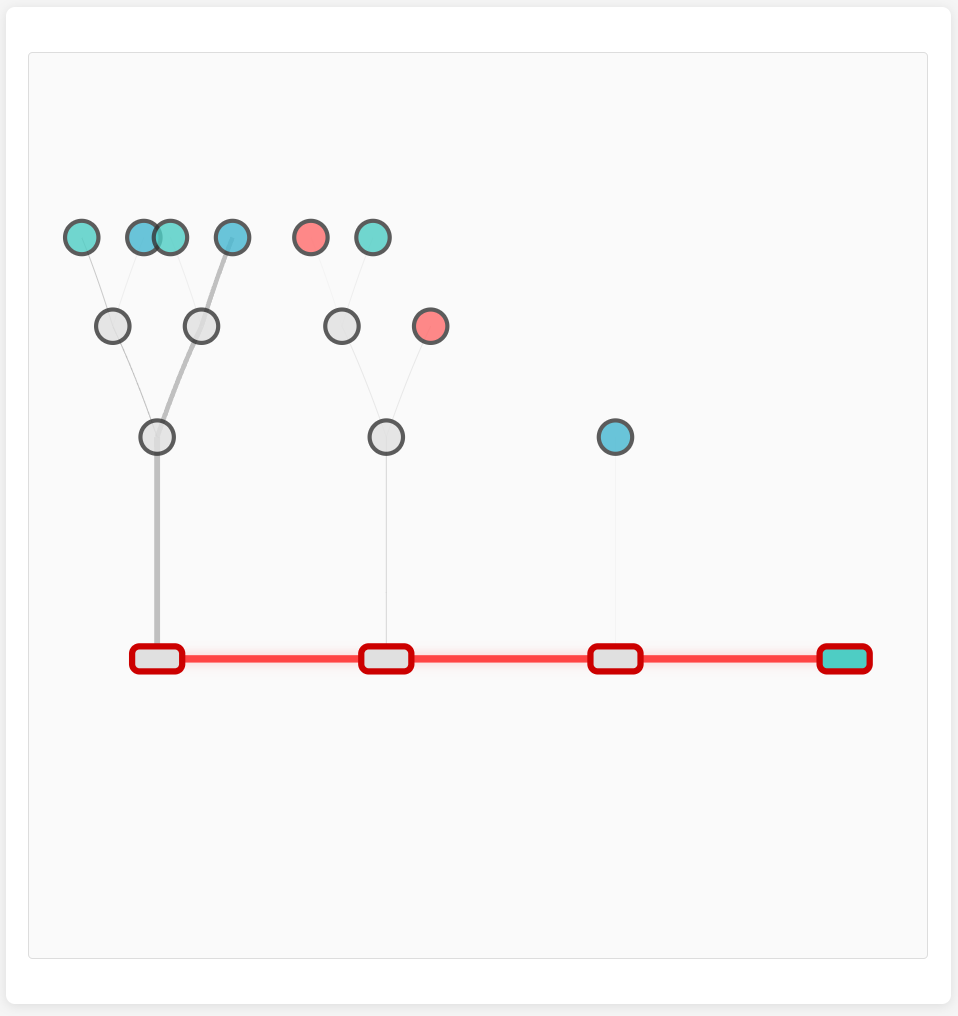
\includegraphics[width=0.45\textwidth]{images/tree spawn 1.png}
    \caption{Rules Centered layout first implementation with rectangular path representation for explained instance path in surrogate model.}
    \label{fig:Tree spawn first implementation}
\end{figure}

Subsequently, text containing the split or label information was added to the rectangular nodes and set to dynamically change according to the size of the rectangle \cite{git29commit}. We implemented functionality for expanding trees not involved in the explained instance path \cite{git30commit}, as one can observe in Figures \ref{fig:collapsedSpawnTree} and \ref{fig:expandedSpawnTree}.

\begin{figure}
    \centering

    \begin{subfigure}[c]{0.45\textwidth}
        \centering
        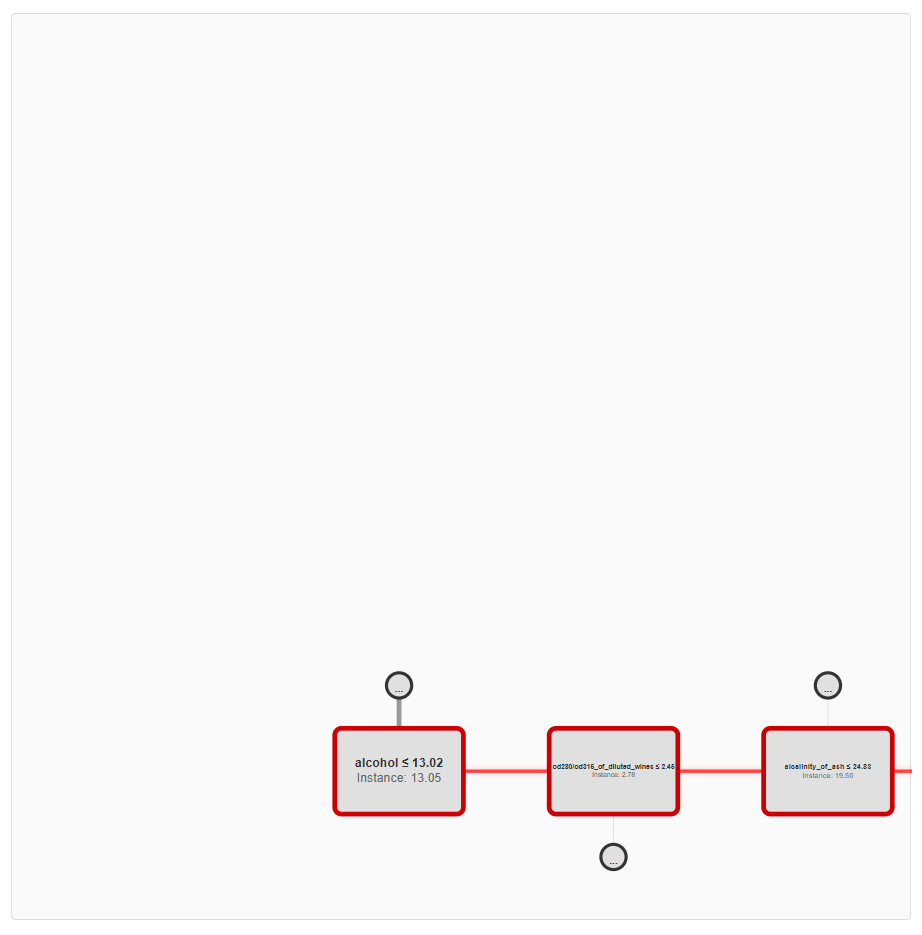
\includegraphics[width=\textwidth]{images/tree spawn v1 collapsed.png}
        \caption{Rules Centered visualization mock up with all collapsed subtrees.}
        \label{fig:collapsedSpawnTree}
    \end{subfigure}
    \hfill
    % Second image
    \begin{subfigure}[c]{0.45\textwidth}
        \centering
        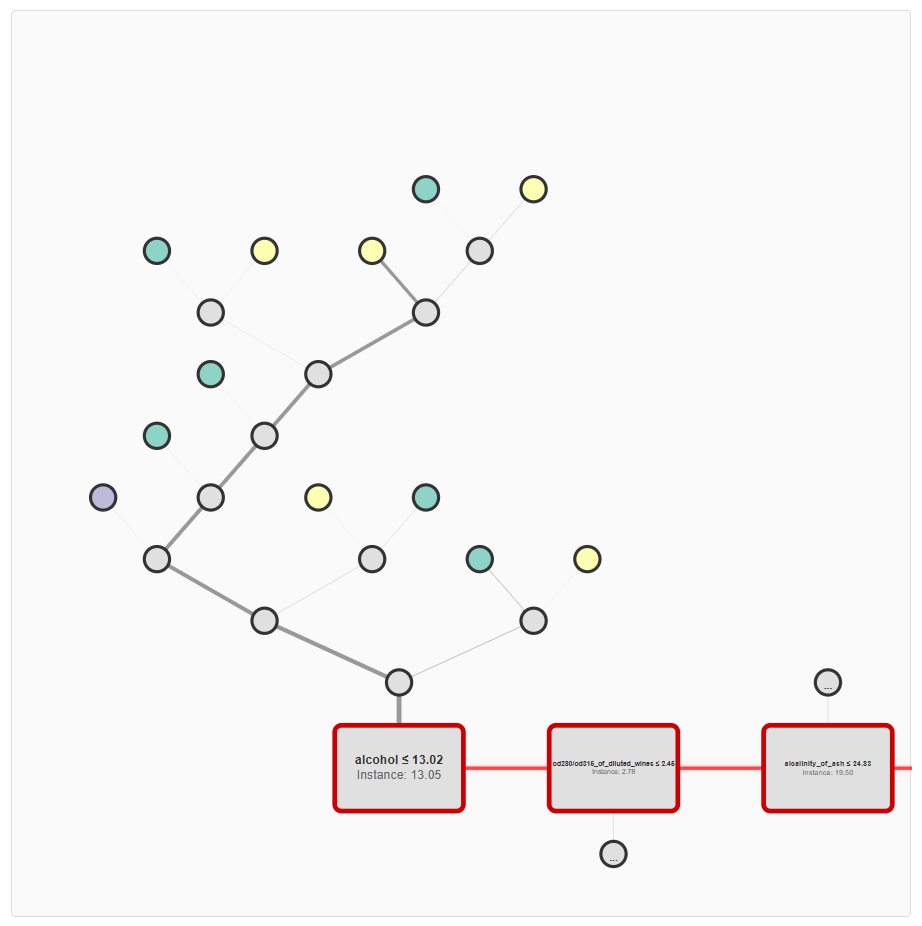
\includegraphics[width=\textwidth]{images/tree spawn v1 expanded.png}
        \caption{Rules Centered visualization mock up with a subtree expanded.}
        \label{fig:expandedSpawnTree}
    \end{subfigure}
    
    \caption{Rules Centered layout visualization with collapsible subtree functionality, demonstrating space-efficient exploration of non-explanation paths through right-click expansion.}
\end{figure}

Following this, we determined spacing between nodes of the explained instance path based on subtree size \cite{git31commit} and integrated the Rules Centered layout implementation into the main interface \cite{git32commit}.

The Rules Centered layout visualization employs a custom linear path layout that fundamentally differs from the hierarchical positioning used in the classic tree visualization. Rather than applying the Reingold-Tilford algorithm to the entire tree structure, the Rules Centered layout visualization uses a hybrid approach that combines linear positioning for the explained instance path with hierarchical layouts for individual subtrees.

The layout algorithm operates in three distinct phases: instance path positioning, subtree size analysis, and off-path subtree placement. Initially, the nodes belonging to the instance path are positioned horizontally along a centerline at $y = h_{inner}/2$, where $h_{inner}$ represents the inner height of the visualization canvas. This horizontal arrangement emphasizes the sequential nature of the decision path and creates a clear visual narrative of how the explained instance traverses the surrogate model.

The horizontal spacing between path nodes is calculated adaptively based on the complexity of off-path subtrees. For each node $n_i$ in the instance path, we compute the total size $s_i$ of all subtrees not on the instance path by recursively counting their descendant nodes. The spacing margin $m_i$ between consecutive path nodes is then determined as shown in Equation \ref{eq:SpawnTreeSpacing}.

\begin{equation}
m_i = m_{base} + s_i \times k_{spacing}
\label{eq:SpawnTreeSpacing}
\end{equation}

where $m_{base} = 100$ pixels represents the minimum separation and $k_{spacing} = 20$ pixels per node is the spacing multiplier. This adaptive approach ensures that larger, more complex subtrees receive proportionally more horizontal space, preventing visual overlap while maintaining efficient space utilization for simpler branches.

To accommodate viewport constraints, we apply a scaling factor when the required width exceeds available space. Given path nodes $\{n_1, n_2, \ldots, n_k\}$ with calculated margins $\{m_1, m_2, \ldots, m_{k-1}\}$, the total required width is $w_{req} = k \times w_{rect} + \sum_{i=1}^{k-1} m_i$, where $w_{rect} = 150$ pixels is the rectangle width. If $w_{req} > w_{available}$, we apply the scaling factor shown in Equation \ref{eq:SpawnTreeScalingFactor}.

\begin{equation}
\alpha = \max\left(0.5, \frac{w_{available} - k \times w_{rect}}{\sum_{i=1}^{k-1} m_i}\right)
\label{eq:SpawnTreeScalingFactor}
\end{equation}

The scaled margins $m_i' = \alpha \times m_i$ are then used to compute final X positions, starting from a centered initial position $x_0 = (w_{available} - w_{final})/2 + w_{rect}/2$, where $w_{final} = k \times w_{rect} + \sum_{i=1}^{k-1} m_i'$.

Off-path subtrees are positioned using the Reingold-Tilford algorithm \cite{1702828}, as previously discussed for the tree layout implementation, independently for each subtree, with their root nodes anchored to their corresponding instance path nodes. The algorithm alternates subtree placement above and below the horizontal path using a global counter, creating a balanced visual distribution. For a subtree rooted at node $t_j$ anchoring to path node $n_i$ at position $(x_i, y_c)$, we first apply D3's tree layout to obtain relative positions. The subtree root is then positioned at $(x_i, y_{anchor})$, where $y_{anchor}$ is determined as shown in Equation \ref{eq:SpawnTreey_anchor}.

\begin{equation}
y_{anchor} = \begin{cases}
y_c - g_{vertical} - d_j & \text{if } j \bmod 2 = 0 \\
y_c + g_{vertical} + d_j & \text{if } j \bmod 2 = 1
\end{cases}
\label{eq:SpawnTreey_anchor}
\end{equation}

Here, $g_{vertical} = 100$ pixels represents the vertical gap between the path and subtrees, and $d_j$ is the vertical extent of subtree $t_j$ from its root. All descendant nodes maintain their relative positions from the D3 layout, preserving the hierarchical structure while integrating with the linear path.

The expand/collapse functionality leverages hierarchical visibility management. Each node maintains state flags: \texttt{isHidden}, \texttt{hasHiddenChildren}, and \texttt{isExpanded}. Initially, subtrees are collapsed beyond a code configurable depth ($d_{initial} = 2$ levels), with nodes deeper than this threshold marked as hidden. Right-clicking a collapsed node triggers the \texttt{expandSubtree} function, which recursively sets \texttt{isHidden = false} for all descendants and updates expansion flags. Conversely, \texttt{collapseSubtree} hides all children and resets their expansion states. The visualization filters links and nodes based on these flags, efficiently managing complex trees by displaying only relevant portions while preserving the complete underlying data structure.

This hybrid approach combines the narrative clarity of linear layouts with the structural fidelity of hierarchical algorithms, creating a visualization that effectively balances explanation-centric design with comprehensive tree exploration capabilities.

\subsubsection{Rule and Counterfactual Rules Centered layout} 
% \label{subsubsec:blocks}

Following the Rules Centered layout visualization development, we realized a first implementation of the Rule and Counterfactual Rules Centred layout \cite{git27commit}, observable in Figure \ref{fig:Blocks tree first implementation}, still using circles for representing the nodes. In this early version, we directed focus toward arranging nodes in the visualization space in the intended way. Subsequently, we developed the first implementation of the Rule and Counterfactual Rules Centered layout using rectangles \cite{git28commit}, which also employed different link stroke widths based on the number of samples passing from one node to the next, as observed in Figure \ref{fig:blocksFirstRect}.

\begin{figure}[ht!]
    \centering
    \begin{subfigure}[c]{0.45\textwidth}
        \centering
        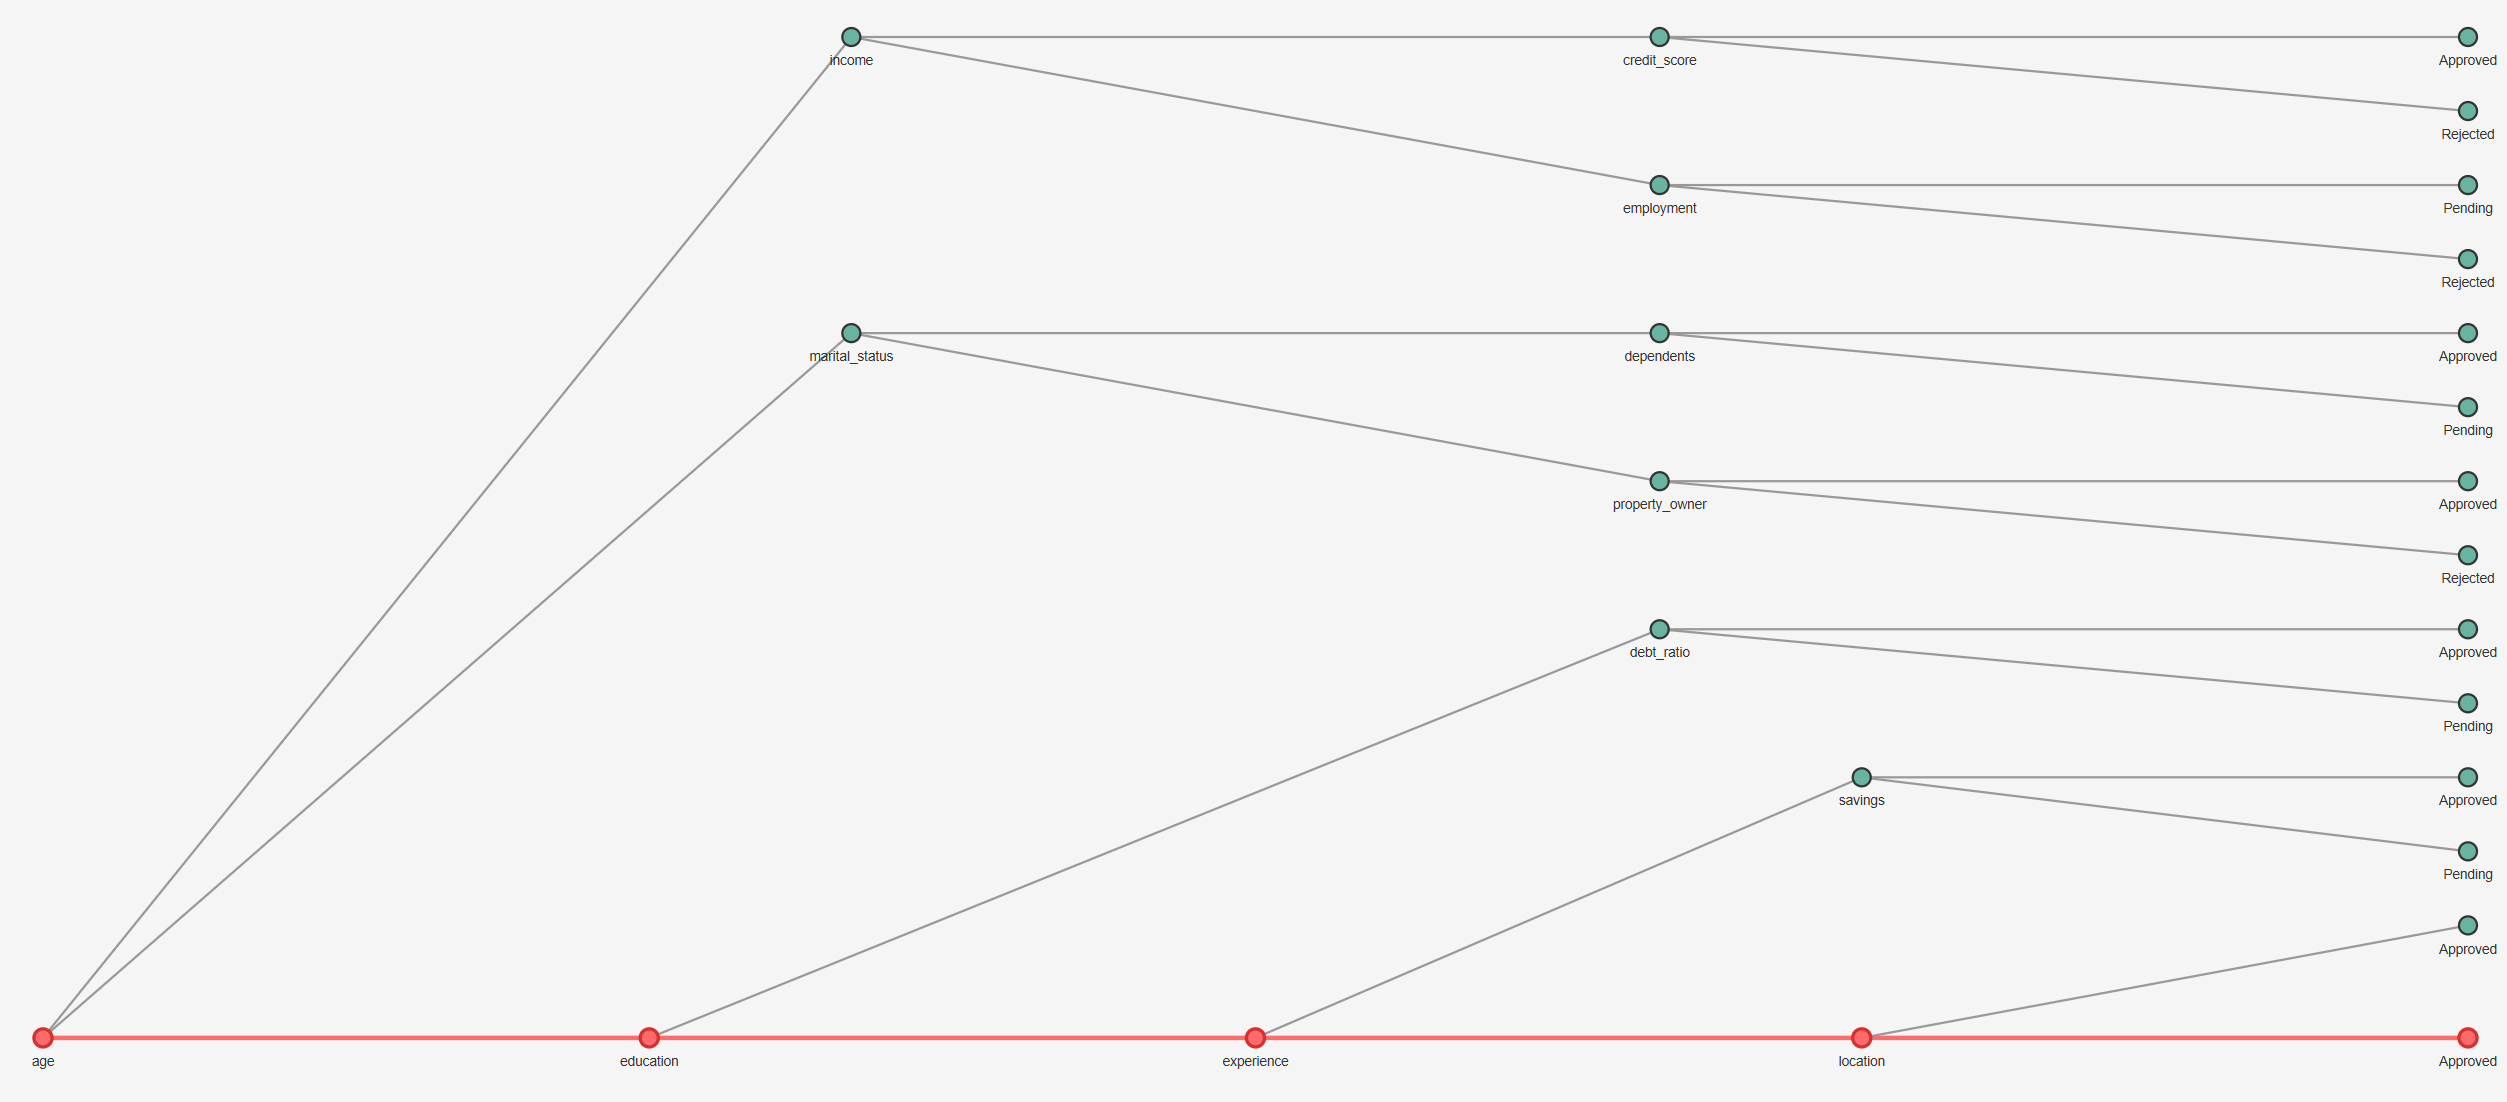
\includegraphics[width=\textwidth]{images/blocks tree skeleton.png}
        \caption{Blocks tree first implementation with focus on nodes arrangement.}
        \label{fig:Blocks tree first implementation}
    \end{subfigure}
    \hfill
    \begin{subfigure}[c]{0.72\textwidth}
        \centering
        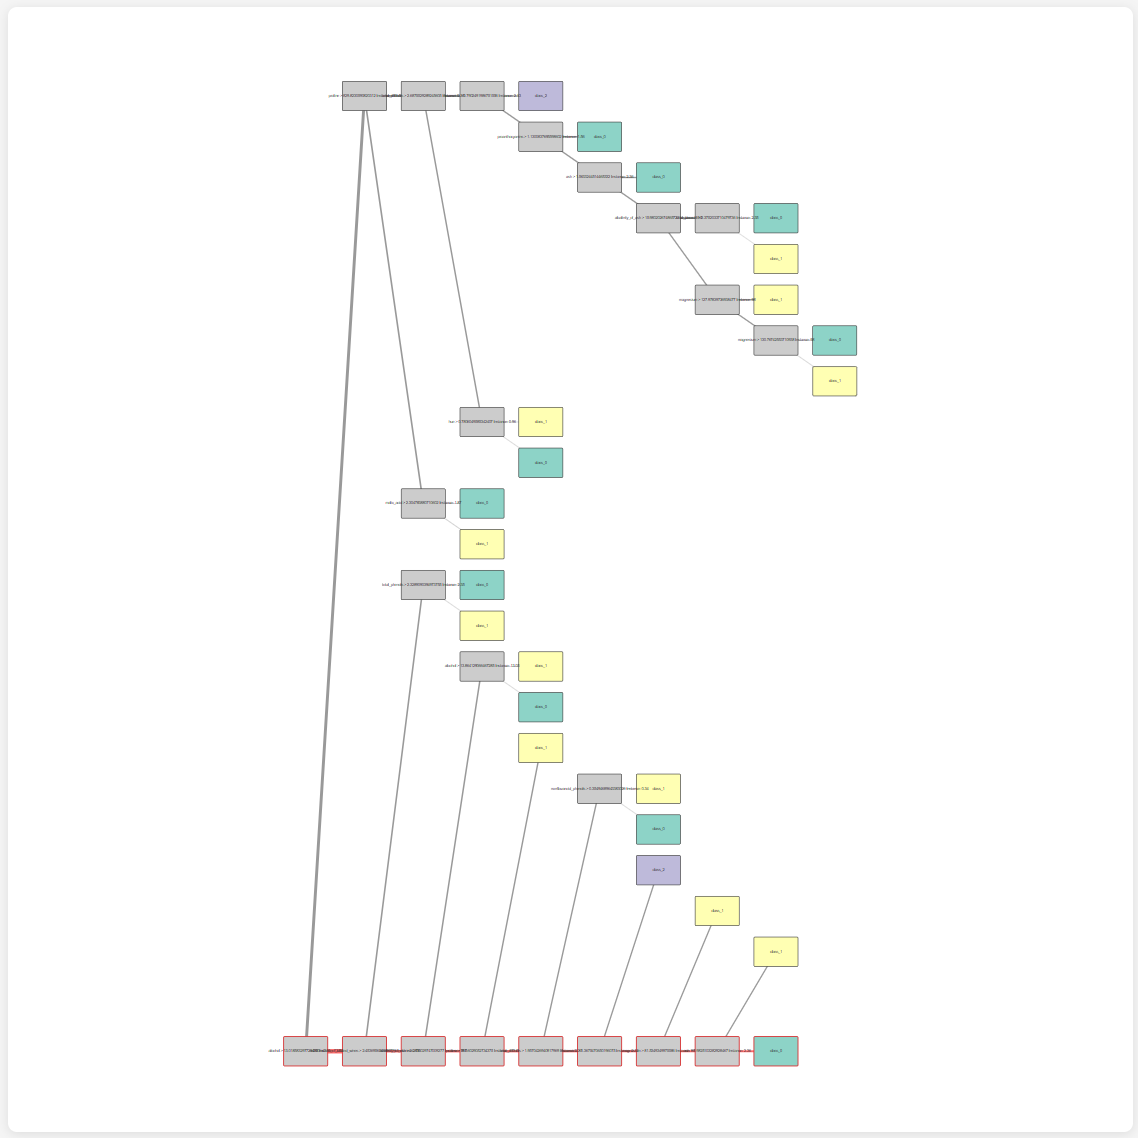
\includegraphics[width=\textwidth]{images/blocks tree first rect.png}
        \caption{Blocks tree first implementation using rectangles.}
        \label{fig:blocksFirstRect}
    \end{subfigure}
    
    \caption{Blocks tree evolution from circular to rectangular nodes with sample-proportional link widths.}
\end{figure}

Subsequently, the font size of rectangular nodes containing text was fixed to dynamically change based on rectangle size \cite{git29commit} for both new visualizations.

The blocks tree visualization employs a depth-aligned layout algorithm that fundamentally departs from hierarchical tree layouts by organizing nodes into vertical columns corresponding to their depth level in the decision tree. This column-based approach prioritizes the sequential nature of decision paths while maintaining clear visual alignment across all branches, facilitating direct comparison of split conditions at equivalent depths.

The layout algorithm is composed of a three-phase positioning strategy: depth column establishment, instance path anchoring, and sorted path distribution. First, the algorithm establishes a uniform horizontal spacing for depth levels by partitioning the available width equally among all depths. For a tree with maximum depth $d_{max}$ and available width $w_{available}$, each depth level $d \in \{0, 1, \ldots, d_{max}\}$ receives a fixed X coordinate as shown in Equation \ref{eq:blocksWidth}.

\begin{equation}
x_d = m_{left} + d \times \frac{w_{available}}{d_{max}}
\label{eq:blocksWidth}
\end{equation}

where $m_{left}$ represents the left margin. This uniform spacing ensures that nodes at the same depth align vertically regardless of their specific path, creating a grid-like structure that emphasizes the decision sequence.

The instance path receives privileged positioning at the bottom of the visualization canvas, anchored at a constant Y coordinate $y_{bottom} = h_{effective} - m_{bottom}$, where $h_{effective}$ is the effective canvas height and $m_{bottom}$ is the bottom margin. This bottom-alignment serves dual purposes: it provides immediate visual identification of the explanation path and creates a stable reference baseline for spatial reasoning about alternative decision paths. Each node $n_i$ in the instance path $\{n_0, n_1, \ldots, n_k\}$ is positioned at coordinates $(x_i, y_{bottom})$, where $x_i$ corresponds to its depth level.

Alternative decision paths are placed above the instance path using a sorting and spacing algorithm that emphasizes their structural relationship to the explanation. The algorithm first identifies all paths not matching the instance path, then sorts these paths by their divergence point from the explained instance. For each alternative path $p$, its branch point $b(p)$ is computed, defined as the index of the last node shared with the instance path as shown in Equation \ref{eq:blocksBranchPoint}.

\begin{equation}
b(p) = \max\{i \mid p[i] = p_{instance}[i], \; 0 \leq i < \min(|p|, |p_{instance}|)\}
\label{eq:blocksBranchPoint}
\end{equation}

Paths are then sorted in ascending order of branch points, ensuring that paths diverging earlier from the instance path appear higher in the visualization, creating a natural visual narrative of progressive specialization toward the explained decision.

The vertical spacing between alternative paths adapts to both the number of paths and the configured node spacing requirements. Given $n_{paths}$ alternative paths and available vertical space $h_{available} = h_{inner} - 2m_{bottom}$, the spacing between consecutive paths is calculated as in Equation \ref{eq:blocksSpacingConsecutive}.

\begin{equation}
s_{path} = \max\left(s_{node}, \frac{h_{available}}{n_{paths}}\right)
\label{eq:blocksSpacingConsecutive}
\end{equation}

where $s_{node}$ represents the minimum acceptable node spacing. This adaptive spacing ensures visual clarity even for complex trees with numerous branches while maintaining sufficient separation for rectangular node dimensions. Each alternative path $p_j$ at sorted index $j$ receives Y coordinate $y_j = m_{top} + j \times s_{path}$, where $m_{top}$ is the top margin.

The blocks layout scales margins dynamically based on tree complexity through a node scale factor $k_{scale} = \max(1, \sqrt{n_{nodes}/100})$, where $n_{nodes}$ represents the total number of unique nodes. All margin values are multiplied by this factor, ensuring that larger trees receive proportionally more spacing while maintaining visual coherence. The effective canvas dimensions are calculated as $w_{effective} = \max(w_{base}, w_{required})$ and $h_{effective} = \max(h_{base}, h_{required})$, where base dimensions represent minimum canvas size and required dimensions account for scaled spacing requirements.

Links between nodes are rendered as straight line segments connecting rectangular node centers, with stroke width proportional to the sample flow through each connection.
% For a link from node $n_i$ to $n_j$ carrying $s_{weighted}$ samples out of $s_{total}$ total samples, the stroke width is calculated as $w_{stroke} = (s_{weighted}/s_{total}) \times 3 \times w_{base}$, where $w_{base}$ is the base link stroke width. This visual encoding of sample distribution provides insight into which branches handle larger portions of the dataset.

The depth-aligned layout offers several analytical advantages compared to traditional hierarchical layouts. The vertical column structure enables direct comparison of decision criteria across branches at equivalent depths, facilitating identification of feature importance patterns and split threshold variations. The bottom-anchored instance path creates a stable visual reference for understanding how the explained decision relates to alternative outcomes, while the sorted arrangement of alternative paths reveals the decision tree's branching structure in relation to the specific instance being explained.

% After implementing these features, the blocks implementation was integrated into the main interface \cite{git33commit}. 
% Subsequently, the integration the two new plots, many bug fixes and small improvements were implemented, along with the implementation in Jupyter Notebook \cite{git34commit}.

